\documentclass[]{book}
\usepackage{lmodern}
\usepackage{amssymb,amsmath}
\usepackage{ifxetex,ifluatex}
\usepackage{fixltx2e} % provides \textsubscript
\ifnum 0\ifxetex 1\fi\ifluatex 1\fi=0 % if pdftex
  \usepackage[T1]{fontenc}
  \usepackage[utf8]{inputenc}
\else % if luatex or xelatex
  \ifxetex
    \usepackage{mathspec}
  \else
    \usepackage{fontspec}
  \fi
  \defaultfontfeatures{Ligatures=TeX,Scale=MatchLowercase}
\fi
% use upquote if available, for straight quotes in verbatim environments
\IfFileExists{upquote.sty}{\usepackage{upquote}}{}
% use microtype if available
\IfFileExists{microtype.sty}{%
\usepackage[]{microtype}
\UseMicrotypeSet[protrusion]{basicmath} % disable protrusion for tt fonts
}{}
\PassOptionsToPackage{hyphens}{url} % url is loaded by hyperref
\usepackage[unicode=true]{hyperref}
\PassOptionsToPackage{usenames,dvipsnames}{color} % color is loaded by hyperref
\hypersetup{
            pdftitle={GxE Fam Project},
            pdfauthor={Andrey Ziyatdinov},
            colorlinks=true,
            linkcolor=Maroon,
            citecolor=Blue,
            urlcolor=Blue,
            breaklinks=true}
\urlstyle{same}  % don't use monospace font for urls
\usepackage{natbib}
\bibliographystyle{apalike}
\usepackage{longtable,booktabs}
% Fix footnotes in tables (requires footnote package)
\IfFileExists{footnote.sty}{\usepackage{footnote}\makesavenoteenv{long table}}{}
\IfFileExists{parskip.sty}{%
\usepackage{parskip}
}{% else
\setlength{\parindent}{0pt}
\setlength{\parskip}{6pt plus 2pt minus 1pt}
}
\setlength{\emergencystretch}{3em}  % prevent overfull lines
\providecommand{\tightlist}{%
  \setlength{\itemsep}{0pt}\setlength{\parskip}{0pt}}
\setcounter{secnumdepth}{5}
% Redefines (sub)paragraphs to behave more like sections
\ifx\paragraph\undefined\else
\let\oldparagraph\paragraph
\renewcommand{\paragraph}[1]{\oldparagraph{#1}\mbox{}}
\fi
\ifx\subparagraph\undefined\else
\let\oldsubparagraph\subparagraph
\renewcommand{\subparagraph}[1]{\oldsubparagraph{#1}\mbox{}}
\fi

% set default figure placement to htbp
\makeatletter
\def\fps@figure{htbp}
\makeatother

\usepackage[sc]{mathpazo}
\usepackage[T1]{fontenc}
\usepackage{geometry}
\geometry{verbose,tmargin=2.5cm,bmargin=2.5cm,lmargin=2.5cm,rmargin=2.5cm}

\usepackage{graphicx}

% copied from bookdown example
% https://github.com/rstudio/bookdown/blob/master/inst/examples/latex/preamble.tex
\usepackage{booktabs}
\usepackage{longtable}
\usepackage[bf,singlelinecheck=off]{caption}

\renewcommand{\textfraction}{0.05}
\renewcommand{\topfraction}{0.8}
\renewcommand{\bottomfraction}{0.8}
\renewcommand{\floatpagefraction}{0.75}

\makeatletter
\newenvironment{kframe}{%
\medskip{}
\setlength{\fboxsep}{.8em}
 \def\at@end@of@kframe{}%
 \ifinner\ifhmode%
  \def\at@end@of@kframe{\end{minipage}}%
  \begin{minipage}{\columnwidth}%
 \fi\fi%
 \def\FrameCommand##1{\hskip\@totalleftmargin \hskip-\fboxsep
 \colorbox{shadecolor}{##1}\hskip-\fboxsep
     % There is no \\@totalrightmargin, so:
     \hskip-\linewidth \hskip-\@totalleftmargin \hskip\columnwidth}%
 \MakeFramed {\advance\hsize-\width
   \@totalleftmargin\z@ \linewidth\hsize
   \@setminipage}}%
 {\par\unskip\endMakeFramed%
 \at@end@of@kframe}
\makeatother

\makeatletter
\@ifundefined{Shaded}{
}{\renewenvironment{Shaded}{\begin{kframe}}{\end{kframe}}}
\makeatother

\title{GxE Fam Project}
\author{Andrey Ziyatdinov}
\date{2018-09-30}

\begin{document}
\maketitle

\setlength{\abovedisplayskip}{-5pt}
\setlength{\abovedisplayshortskip}{-5pt}

{
\hypersetup{linkcolor=black}
\setcounter{tocdepth}{2}
\tableofcontents
}
\chapter*{Preface}\label{preface}
\addcontentsline{toc}{chapter}{Preface}

Links

\begin{itemize}
\tightlist
\item
  Public version of the book:
  \href{https://hemostat.github.io/Public/Papers/05-int-rel/bookdown/index.html}{html},
  \href{https://hemostat.github.io/Public/Papers/05-int-rel/bookdown/gxefam.pdf}{pdf},
  \href{https://hemostat.github.io/Public/Papers/05-int-rel/bookdown/gxefam.docx}{docx},
  \href{https://raw.githubusercontent.com/hemostat/Public/gh-pages/Papers/05-int-rel/bookdown/gxefam.md}{md},
  \href{https://hemostat.github.io/Public/Papers/05-int-rel/bookdown/gxefam.tex}{tex}
\end{itemize}

\chapter{Manuscript}\label{manuscript}

\textbf{Title}: Statistical power in GWAS revisited: effective sample
size, genetic relatedness, and gene-by-environment interactions

\textbf{Title 2}: Advantages and limitations of linear mixed model in
genetic association studies

\textbf{Abstract}: Genome-wide association studies (GWAS) have
identified thousands of genetic variants associated with complex
diseases and~ heavily rely on increasing the sample size. Recent
analyses of biobank-scale genetic data suggest: (i) inclusion of
genetically related individuals empowers GWAS \citep{loh2018mixed}; (ii)
the wealth of collected environmental exposures has potential to uncover
gene-by-environmental interactions \citep{young2016multiple}. However,
quantification of GWAS power ---~ the non-centrality parameter (\(NCP\))
of association test, which is proportional to the sample size (\(n\))
and the variance explained by genetic variant (\(q^2\)) ---~ holds only
for unrelated individuals. Here, we first expanded it by
incorporating~individual relationships by linear mixed model. We next
studied~gene-by-environment interactions, where interaction effect on
trait is tested in the presence of marginal genetic effect. In result,
the derived formulas have a range of implications. For testing marginal
genetic~effect, one can~quickly assess the power in studies involving
related individuals. Because of the potential gain in power for
testing~gene-by-environment interaction, the formula~for interactions
will allow optimization of the study design of related individuals.

\section{Introduction}\label{introduction}

The vast majority of genome-wide association studies (GWAS) conducted so
far has used standard fixed effect models. This strategy has been showed
to be at the same time robust and fast, allowing for the analysis of
thousands of individuals and millions of genetic variants in a
reasonable computation time. However, in parallel, there has been
increased interest in using linear mixed model (LMM) for the purpose of
genome-wide association mapping. LMM has been considered for several
reasons. Random effects models have primarily been used to control for
the type I error rate account when analyzing related individuals.
Indeed, when not modeled, genetic relationship will in general lead to
an underestimation of the effect estimates, thus producing inflated
statistics. LMM has also been showed to be of interest for increasing
power, and because of that, there has been increasing literature about
the possibility of using LMM more systematically in GWAS {[}ref{]}.
However, LMM have also limitation, including in particular a dramatic
increase in computation time, making the approach intractable for
extremely large sample size, or when analyzing multiple phenotypes
{[}ref{]}. \ldots{} other issues \ldots{}. Overall, many issues have
been solved, and LMM will likely be increasingly used in GWAS settings
by the community. However, the expected gain in power that one might
achieve relative to the computational cost of LMM has not been solved.

Here, we proposed an analytical framework

Previous studies already discussed the ability of LMM to prevent false
positive associations due to population stratification, how to reduce
the computational burden of LMM {[}ref{]}, and potential gain in power
that might be achieved

However the later

How the 2 combine both\ldots{}

\section{Methods and Analytical
Derivations}\label{methods-and-analytical-derivations}

\subsection{Linear mixed model for genetic association
study}\label{linear-mixed-model-for-genetic-association-study}

We consider the following linear mixed model to study the impact of
relatedness among individuals on modeling a continuous phenotype \(y\).

\begin{equation}
  y = X \beta + \sum_{k=1}^{m}{r_k} + e
\label{eq:assoclmm}
\end{equation}

where \(n\) is the number of individuals, \(p\) is the number of
covariates or fixed effects, \(m\) is the number of structured random
effects apart from the residuals errors, \(y\) is a phenotype vector of
length \(n\), \(X\) is a matrix of covariates of size \(n \times p\),
\(\beta\) is a vector of fixed effects of length \(p\). The vectors of
random effects \(r_k\) and \(e\) are mutually uncorrelated and
multivariate normally distributed as \(\mathcal{N}(0, \sigma^2_k R_k)\)
and \(\mathcal{N}(0, \sigma^2_r I)\). The variance-covariance matrices
are parametrized with scalar parameters (referred as variance
components) and constant matrices of size \(n \times n\) that express
relationships among \(n\) individuals. The first \(m\) random effects
\(r_k\) are referred here as structured, whereas the last component
\(e\) is simply the residual errors which are independent and
identically distributed.

Thus, the phenotype follows a multivariate normal distribution (MVN) and
Equation \eqref{eq:assoclmm} can be rewritten:

\begin{equation}
  y \sim \mathcal{N} (X \beta, V) = \mathcal{N} (X \beta, \sum_{k=1}^{m}{\sigma_k^2 R_k} + \sigma_r^2 I) 
\label{eq:assocmvn}
\end{equation}

An assosiation test for a given variable in the matrix \(X\) consists in
constructing the score test statistic based on the estimates of effect
size and its variance,
\(Z = \hat{\beta}_x / \sqrt{var(\hat{\beta}_x)}\). The score follows the
standard normal distribution \(Z \sim \mathcal{N}(0, 1)\), and the
\(\chi^2\) test with non-centrality parameter
\(NCP = \beta^2_x / var(\hat{\beta}_x)\) quantifies the statistical
power for a given true effect size \(\beta_x\).

We further consider several parameterizations of the model in Equation
\eqref{eq:assocmvn} that depend on (i) whether marginal genetic or
gene-environment interaction effect is under testing; (ii) whether
structured random effects are included or only the residual errors are
present. The detailed derivation of the formulas presented next is given
in Supplementary Material, Section \ref{derivations}.

We introduce common assumptions and notations before going further. We
assume that all vectors of the phenotype (\(y\)) and covariates (columns
in the matrix \(X\)) are centered. The phenotype vector is additionally
standardized (\(var(y) = 1\)). The genotype vector \(x_g\) is considered
as a realization of a vector of random variables \(\mathcal{X_g}\),
which is a genotype in \(n\) individuals with a minor allele frequency
\(p\). We denote the distribution
\(\mathcal{X_g} \sim (\mu_g, \Sigma_g) = (p 1_n, \delta_g^2 K) = (p 1_n, 2 p (1-p) K)\),
where \(K\) is the kinship matrix of size \(n \times n\) (it can be the
identity matrix \(I\) for genetically unrelated individuals) and \(1_n\)
is a vector of \(n\) ones.

\subsection{Testing marginal genetic
effect}\label{testing-marginal-genetic-effect}

The genetic effect on phenotype in unrelated individuals is evaluated
under the standard linear model
\(y \sim \mathcal{N} (\mu x_0 + \beta_g x_g, \sigma_r^2 I)\), where
\(x_0 = 1_n\) is a vector of \(n\) ones, \(\mu\) is a mean of the
phenotypic values, \(x_g\) is a vector of length of the genotypic
values, \(\beta_g\) is the effect size of the genotype. The NCP
parameter of the test in linear model is well known to be proportional
to the sample size and the variance captured by the genotype (see also
Section \ref{lmg}).

\begin{equation}
NCP_{unrel} \approx \beta_g^2 \delta_g^2 n  = \hat{\beta}_g^2 2 p (1 - p) n
\label{eq:ncpgun}
\end{equation}

When the individuals are genetically related and/or the covariance of
the phenotype is modeled using structured relationship matrices among
individuals, the following linear mixed model is stated,
\(y \sim \mathcal{N} (\mu x_0 + \beta_g x_g, \sum_{k=1}^{m}{\sigma_k^2 R_k} + \sigma_r^2 I)\).
The initial step in solving a linear mixed model is to estimate random
effects parameters (\(\sigma_k^2\) and \(\sigma_r^2\)) by restricted
maximum likelihood (REML) or other optimization technique
\citep{Lynch1998}. Once the estimate of the variance-covariance matrix
is found, \(\hat{V} = \sum{\hat{\sigma}_i^2 R_i} + \hat{\sigma}_r^2 I\),
the generalized least squares (GLS) for fixed effects are applied in the
following matrix form,
\(\hat{\beta} = \left(X^T \hat{V}^{-1} X\right)^{-1} X \hat{V}^{-1} y\).

In Section \ref{lmmg} we derived the estimate of \(\beta_g\) and its
variance,
\(\hat{\beta}_g = \left(\tilde{x}_g^T \hat{V}^{-1} \tilde{x}_g\right)^{-1} \tilde{x}_g^T \hat{V}^{-1} \tilde{y}\)
and
\(var(\hat{\beta_g}) = 1 / (\tilde{x}_g^T \hat{V}^{-1} \tilde{x}_g)\),
respectively. We further approximated the term
\(\tilde{x}_g^T \hat{V}^{-1} \tilde{x}_g\) using the expected mean of a
quadratic form of the random variable \(\mathcal{\tilde{X}_g}\) and the
transformation matrix \(\hat{V}^{-1}\) (see Equation
\eqref{eq:quadform1}). The NCP parameter of the test in linear mixed model
has the following form, where \(tr\) denote the trace operator.

\begin{equation}
NCP_{rel} \approx beta_g^2 tr(\hat{V}^{-1} \Sigma_g) = \beta_g^2 \delta_g^2 tr(\hat{V}^{-1} K) = \beta_g^2 2 p (1 - p) tr(\hat{V}^{-1} K)
\label{eq:ncpgrel}
\end{equation}

The effective size multiplier, defined as \(NCP_{rel} / NCP_{unrel}\),
gives a quantitative assessment of gain or loss in power when comparing
the study design of related and unrelated individuals.

\begin{equation}
NCP_{rel} / NCP_{unrel} = tr(\hat{V}^{-1} K) / n
\label{eq:ncpg}
\end{equation}

We further expand Equation \eqref{eq:ncpgrel} for two specific cases of
(i) related individuals in families; (ii) unrelated individuals under
the the infinite-testimal model. We also make use of the connection
between the trace operator and eigen-value decomposition (Section
\ref{propositions}).

For individuals in families and the model
\(y \sim \mathcal{N} (\mu x_0 + \beta_g x_g, \sigma_k^2 K + \sigma_r^2 I)\),
we have an updated formula of \(NCP_{ref}\).

\begin{equation}
\begin{split}
NCP_{fam} & = \beta_g^2 2 p (1 - p) tr \left( \left(\hat{\sigma}_k^2 K + \hat{\sigma}_r^2 I\right)^{-1} K \right)  \\
 & = \beta_g^2 2 p (1 - p) tr \left( \left(\hat{\sigma}_k^2 I + \hat{\sigma}_r^2 K^{-1}\right)^{-1} \right) \\
 & = \beta_g^2 2 p (1 - p) \sum_{i=1}^{n}{\left(\hat{\sigma}_k^2 + \hat{\sigma}_r^2 \left(\lambda_{K}^i\right)^{-1}\right)^{-1}}
\end{split}
\label{eq:ncpgfam}
\end{equation}

When modeling the polygenic effect in unrelated individuals using the
genetic relationship matrix (GRM) (denoted as \(M\) in equations)
\(y \sim \mathcal{N} (\mu x_0 + \beta_g x_g, \sigma_m^2 M + \sigma_r^2 I)\),
we rewrite \(NCP_{ref}\) as following.

\begin{equation}
\begin{split}
NCP_{unrel+grm} & = \beta_g^2 2 p (1 - p) tr( (\hat{\sigma}_k^2 M + \hat{\sigma}_r^2 I)^{-1} )  \\
 & = \beta_g^2 2 p (1 - p) \sum_{i=1}^{n}{(\hat{\sigma}_m^2 \lambda_{M}^i + \hat{\sigma}_r^2)^{-1}}
\end{split}
\label{eq:ncpggrm}
\end{equation}

\subsection{Testing gene-environment interaction
effect}\label{testing-gene-environment-interaction-effect}

The gene-environment interaction effect on phenotype in unrelated
individuals is evaluated under the standard linear model
\(y \sim \mathcal{N} (\mu x_0 + \beta_g x_g + \beta_e x_e + \beta_{ge} x_{ge}, \sigma_r^2 I)\),
where \(x_0 = 1_n\) is a vector of \(n\) ones, \(\mu\) is a mean of the
phenotypic values, \(x_g\) is a vector of length of the genotypic
values, \(\beta_g\) is the effect size of the genotype, \(x_e\) is a
environment exposure vector of length \(n\), \(\beta_e\) is the effect
size of the environment exposure, \(x_{ge}\) is a vector of length \(n\)
of gene-environment interaction, \(\beta_{ge}\) is the interaction
effect size.

The coding scheme of the genotypic and environmental variables to study
gene-environment interaction under linear model is important and has
been reviewed elsewhere \citep{Aschard2016}. Here, we work with centered
variables \(\tilde{x}_g\) and \(\tilde{x}_e\) and define the interaction
variable \(\tilde{x}_{ge}\) by (i) element-wise multiplication of the
two variables, (ii) centering the resulted product. Once the covariates
are centered as described above, the effect sizes and their standard
errors can be estimated independently from other covariates if we assume
that the two random variables of genotype and environmental exposure are
generated independently \citep[Appendix C]{Aschard2016}. We also note
that different coding schemes give different estimates of effect sizes,
but the test statistic for gene-environment interaction (\(NCP\)) is the
same \citep[Appendix B]{Aschard2016}.

We first need to define two matrices \(E\) and \(D\). The matrix \(E\)
is related to the environment exposure (centered) vector
\(\tilde{x}_e\): \(E\) is the diagonal matrix with values equal to those
observed in \(\tilde{x}_e\), i.e. \(diag(E) = \tilde{x}_e\). We also
introduce a matrix \(D\), which value at row \(i\) and column \(j\) is
equal to the product of two diagonal entries \(i\) and \(j\) of \(E\),
i.e. \(D_{i,j} = E_{i,i} E_{j,j}\). When the environmental exposure is
binary and the observed frequency of exposure is \(f\), then we denote
the matrices as \(E_b\) and \(D_b\). Then the values on diagonal of the
matrix \(E_b\) are either \(-f\) or \(1 - f\), while values of the
matrix \(D_b\) are either \(f^2\), \((1 - f)^2\) or \(f (1 - f)\).

Then the NCP parameter of the test in linear model has the following
form (see Section \ref{lmmge}).

\begin{equation}
NCP_{unrel}^i \approx \beta_{ge}^2 \delta_g^2 tr(E_b^2) = \beta_{ge}^2 2 p (1 - p) f (1 - f) n 
\label{eq:ncpgeun}
\end{equation}

When the individuals are genetically related and/or relationships among
individuals are modeled, we again use the linear mixed model
\(y \sim \mathcal{N} (\mu x_0 + \beta_g x_g + \beta_e x_e + \beta_{ge} x_{ge}, \sum_{k=1}^{m}{\sigma_k^2 R_k} + \sigma_r^2 I)\).

In Section \ref{lmmge} we derived the estimate of \(\beta_{ge}\) and its
variance for linear mixed model,
\(\hat{\beta}_{ge} = \left(\tilde{x}_{ge}^T \hat{V}^{-1} \tilde{x}_{ge}\right)^{-1} \tilde{x}_{ge}^T \hat{V}^{-1} \tilde{y}\)
and
\(var(\hat{\beta_{ge}}) = 1 / (\tilde{x}_{ge}^T \hat{V}^{-1} \tilde{x}_{ge})\),
respectively. As \(\tilde{x}_{ge}\) is a realization of a random
variable \(\mathcal{\tilde{X}}_{ge} = E \mathcal{\tilde{X}}_{g}\), we
showed that \(var(\mathcal{\tilde{X}}_{ge}) = \delta_g^2 D \circ K\).

Here, we introduce a special kinship matrix \(K_{D}\) ``masked'' by the
(observed) environmental exposure though the matrix \(D\) (the operator
\(\circ\) denotes the Hadamard product, i.e.~the element-wise
multiplication).

\begin{equation}
\begin{split}
K_{D} =  D \circ K
\end{split}
\label{eq:kdmat}
\end{equation}

In Section \ref{lmmge} we further approximated the term
\(\tilde{x}_{ge}^T \hat{V}^{-1} \tilde{x}_{ge}\) by applying the
expression for the mean of a quadratic form of the random variable
\(\mathcal{\tilde{X}_{ge}}\) and the transformation matrix
\(\hat{V}^{-1}\) (see Equation \eqref{eq:quadform1}). The NCP parameter of
the test in linear mixed model has the following form.

\begin{equation}
NCP_{rel}^i \approx \beta_{ge}^2 \delta_g^2 tr(\hat{V}^{-1} K_{D}) = \beta_{ge}^2 2 p (1 - p) tr(\hat{V}^{-1} K_{D})
\label{eq:ncpgerel}
\end{equation}

The \(K_{D}\) matrix is equal to the \(E^2\) matrix in the case of
genetically unrelated individuals (\(K = I\)), and the two formulas
\eqref{eq:ncpgerel} and \eqref{eq:ncpgeun} become the same. We also note
that the variance of the environmental exposure is contained within the
matrices \(K_{D}\) and \(E^2\), although it is possible to similarly
define the scaled matrices.

TODO: \(V = \sigma^2_k K + \sigma^2_i K^i + \sigma^2_r I\)
\citep{Sul2016}

\section{Results}\label{results}

\subsection{Analytical results for testing marginal genetic
effect}\label{analytical-results-for-testing-marginal-genetic-effect}

\begin{longtable}[]{@{}llll@{}}
\caption{\label{tab:assoc-gen} Analytical comparison of study designs to
detect marginal genetic association. Study designs differ in individual
relationships that informs modeling of outcome (\(y\)) and distribution
of genotype under association test (\(x_g\)). Study designs under
comparison include: unrelated individuals; related individuals in
families; unrelated individuals with a grouping factor such as
house-hold (not related to a variable under test). Notation:
\(\tilde{x_g}\), mean-centered genotype vector \(x_g\);
\(\delta_g^2 = 2 p (1 - p)\), the variance of genotype random variable
with the minor allele frequency \(p\); \(K\), the additive kinship
matrix for family-based study design; \(NCP\), the non-centrality
parameter of the test; \(\hat{V}\), the estimated variance-covariance
matrix of \(y\).}\tabularnewline
\toprule
\begin{minipage}[b]{0.21\columnwidth}\raggedright\strut
Study design\strut
\end{minipage} & \begin{minipage}[b]{0.15\columnwidth}\raggedright\strut
\(V = Var(y)\)\strut
\end{minipage} & \begin{minipage}[b]{0.16\columnwidth}\raggedright\strut
\(\Sigma_g = Var(\mathcal{\tilde{X}}_g)\)\strut
\end{minipage} & \begin{minipage}[b]{0.37\columnwidth}\raggedright\strut
\(NCP\)\strut
\end{minipage}\tabularnewline
\midrule
\endfirsthead
\toprule
\begin{minipage}[b]{0.21\columnwidth}\raggedright\strut
Study design\strut
\end{minipage} & \begin{minipage}[b]{0.15\columnwidth}\raggedright\strut
\(V = Var(y)\)\strut
\end{minipage} & \begin{minipage}[b]{0.16\columnwidth}\raggedright\strut
\(\Sigma_g = Var(\mathcal{\tilde{X}}_g)\)\strut
\end{minipage} & \begin{minipage}[b]{0.37\columnwidth}\raggedright\strut
\(NCP\)\strut
\end{minipage}\tabularnewline
\midrule
\endhead
\begin{minipage}[t]{0.21\columnwidth}\raggedright\strut
Unrelated\strut
\end{minipage} & \begin{minipage}[t]{0.15\columnwidth}\raggedright\strut
\(\sigma_r^2 I\)\strut
\end{minipage} & \begin{minipage}[t]{0.16\columnwidth}\raggedright\strut
\(\delta_g^2 I\)\strut
\end{minipage} & \begin{minipage}[t]{0.37\columnwidth}\raggedright\strut
\(\beta^2_g (\tilde{x_g}^T \tilde{x_g}) \approx \beta^2_g \delta_g^2 n\)\strut
\end{minipage}\tabularnewline
\begin{minipage}[t]{0.21\columnwidth}\raggedright\strut
Families\strut
\end{minipage} & \begin{minipage}[t]{0.15\columnwidth}\raggedright\strut
\(\sigma_k^2 K + \sigma_r^2 I\)\strut
\end{minipage} & \begin{minipage}[t]{0.16\columnwidth}\raggedright\strut
\(\delta_g^2 K\)\strut
\end{minipage} & \begin{minipage}[t]{0.37\columnwidth}\raggedright\strut
\(\beta^2_g (\tilde{x_g}^T \hat{V}^{-1} \tilde{x_g}) \approx \beta^2_g \delta_g^2 \mbox { } tr(\hat{V}^{-1} K)\)\strut
\end{minipage}\tabularnewline
\begin{minipage}[t]{0.21\columnwidth}\raggedright\strut
Unrelated + Grouping\strut
\end{minipage} & \begin{minipage}[t]{0.15\columnwidth}\raggedright\strut
\(\sigma_h^2 H + \sigma_r^2 I\)\strut
\end{minipage} & \begin{minipage}[t]{0.16\columnwidth}\raggedright\strut
\(\delta_g^2 I\)\strut
\end{minipage} & \begin{minipage}[t]{0.37\columnwidth}\raggedright\strut
\(\beta^2_g (\tilde{x_g}^T \hat{V}^{-1} \tilde{x_g}) \approx \beta^2_g \delta_g^2 \mbox { } tr(\hat{V}^{-1})\)\strut
\end{minipage}\tabularnewline
\bottomrule
\end{longtable}

\begin{figure}

{\centering 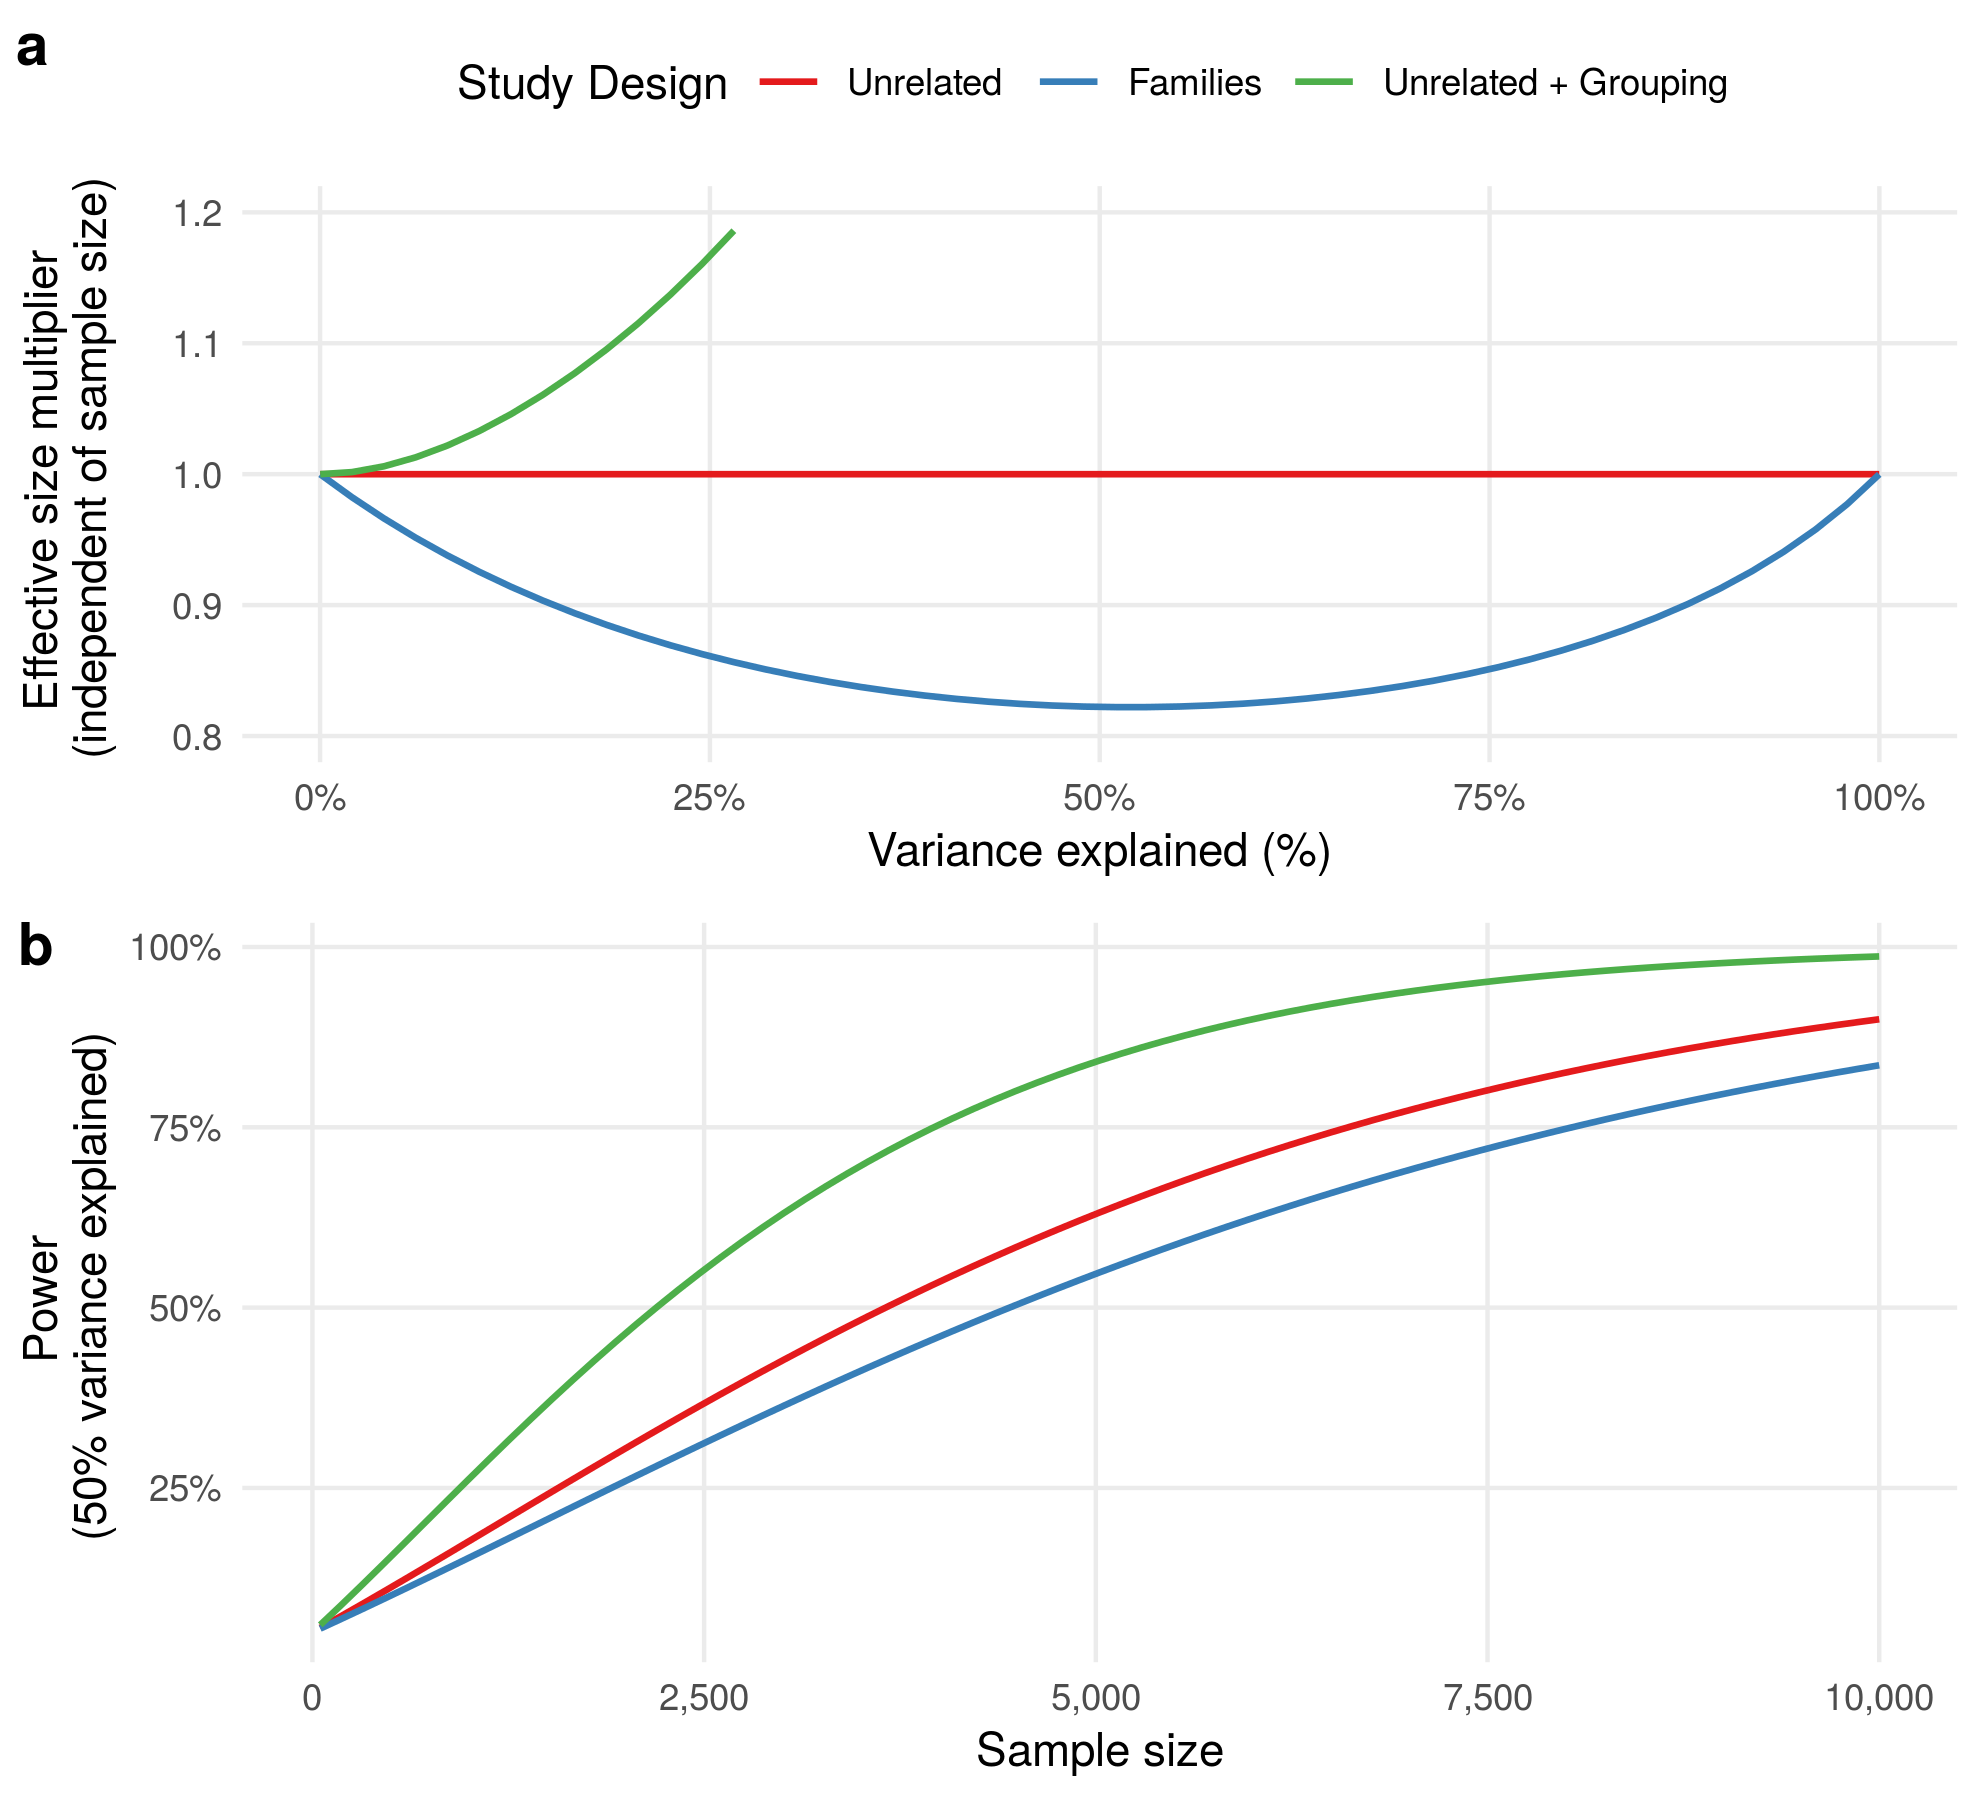
\includegraphics[width=0.75\linewidth]{figures/07-figure-power-marginal-two-panels} 

}

\caption{Three study designs are compared in terms of power
to detect marginal genetic effect under the model
\(y \sim \mathcal{N}(\mu + \beta_g x_g, V)\) (see also Table
\ref{tab:assoc-gen}). The reference study design ``Unrelated'' with
\(V = \sigma^2_r I\) is; the study}\label{fig:power-marginal}
\end{figure}







Two study designs with a structured variance components, unrelated
individuals with a non-genetic grouping factor and related individuals
in families, are compared to the reference study design of unrelated
individuals. The performance is evaluated to To make the study designs
comparable, the sum of variance components in the \(V\) matrix is equal
to one. (a) The effective size multiplier, estimated as
\(tr(V^{-1} \Sigma_g) / n\), depends on the variance explained. (b) When
the variance explained fixed to 50\% and the sample size varies,
Notation: \(n\), the sample size.

Ref \ref{fig:power-marginal}

\subsection{Analytical results for testing gene-environment interaction
effect}\label{analytical-results-for-testing-gene-environment-interaction-effect}

\begin{longtable}[]{@{}llll@{}}
\caption{\label{tab:assoc-ge} Analytical comparison of study designs to
detect gene-environment interaction association.}\tabularnewline
\toprule
\begin{minipage}[b]{0.15\columnwidth}\raggedright\strut
Study design\strut
\end{minipage} & \begin{minipage}[b]{0.16\columnwidth}\raggedright\strut
\(V = Var(y)\)\strut
\end{minipage} & \begin{minipage}[b]{0.17\columnwidth}\raggedright\strut
\(\Sigma_{ge} = Var(E \mathcal{\tilde{X}}_g)\)\strut
\end{minipage} & \begin{minipage}[b]{0.40\columnwidth}\raggedright\strut
\(NCP\)\strut
\end{minipage}\tabularnewline
\midrule
\endfirsthead
\toprule
\begin{minipage}[b]{0.15\columnwidth}\raggedright\strut
Study design\strut
\end{minipage} & \begin{minipage}[b]{0.16\columnwidth}\raggedright\strut
\(V = Var(y)\)\strut
\end{minipage} & \begin{minipage}[b]{0.17\columnwidth}\raggedright\strut
\(\Sigma_{ge} = Var(E \mathcal{\tilde{X}}_g)\)\strut
\end{minipage} & \begin{minipage}[b]{0.40\columnwidth}\raggedright\strut
\(NCP\)\strut
\end{minipage}\tabularnewline
\midrule
\endhead
\begin{minipage}[t]{0.15\columnwidth}\raggedright\strut
Unrelated\strut
\end{minipage} & \begin{minipage}[t]{0.16\columnwidth}\raggedright\strut
\(\sigma_r^2 I\)\strut
\end{minipage} & \begin{minipage}[t]{0.17\columnwidth}\raggedright\strut
\(\delta_g^2 E^2\)\strut
\end{minipage} & \begin{minipage}[t]{0.40\columnwidth}\raggedright\strut
\(\beta^2_{ge} (\tilde{x_{ge}}^T \tilde{x_{ge}}) \approx \beta^2_{ge} \delta_g^2 tr(E^2)\)\strut
\end{minipage}\tabularnewline
\begin{minipage}[t]{0.15\columnwidth}\raggedright\strut
Unrelated (binary)\strut
\end{minipage} & \begin{minipage}[t]{0.16\columnwidth}\raggedright\strut
\(\sigma_r^2 I\)\strut
\end{minipage} & \begin{minipage}[t]{0.17\columnwidth}\raggedright\strut
\(\delta_g^2 E_b^2\)\strut
\end{minipage} & \begin{minipage}[t]{0.40\columnwidth}\raggedright\strut
\(\beta^2_{ge} (\tilde{x_{ge}}^T \tilde{x_{ge}}) \approx \beta^2_{ge} \delta_g^2 f (1 -f) n\)\strut
\end{minipage}\tabularnewline
\begin{minipage}[t]{0.15\columnwidth}\raggedright\strut
Families\strut
\end{minipage} & \begin{minipage}[t]{0.16\columnwidth}\raggedright\strut
\(\sigma_k^2 K + \sigma_i^2 K_i + \sigma_r^2 I\)\strut
\end{minipage} & \begin{minipage}[t]{0.17\columnwidth}\raggedright\strut
\(\delta_g^2 K_D\)\strut
\end{minipage} & \begin{minipage}[t]{0.40\columnwidth}\raggedright\strut
\(\beta^2_{ge} (\tilde{x_{ge}}^T \hat{V}^{-1} \tilde{x_{ge}}) \approx \beta^2_{ge} \delta_g^2 \mbox { } tr(\hat{V}^{-1} K_D)\)\strut
\end{minipage}\tabularnewline
\bottomrule
\end{longtable}

\begin{figure}

{\centering 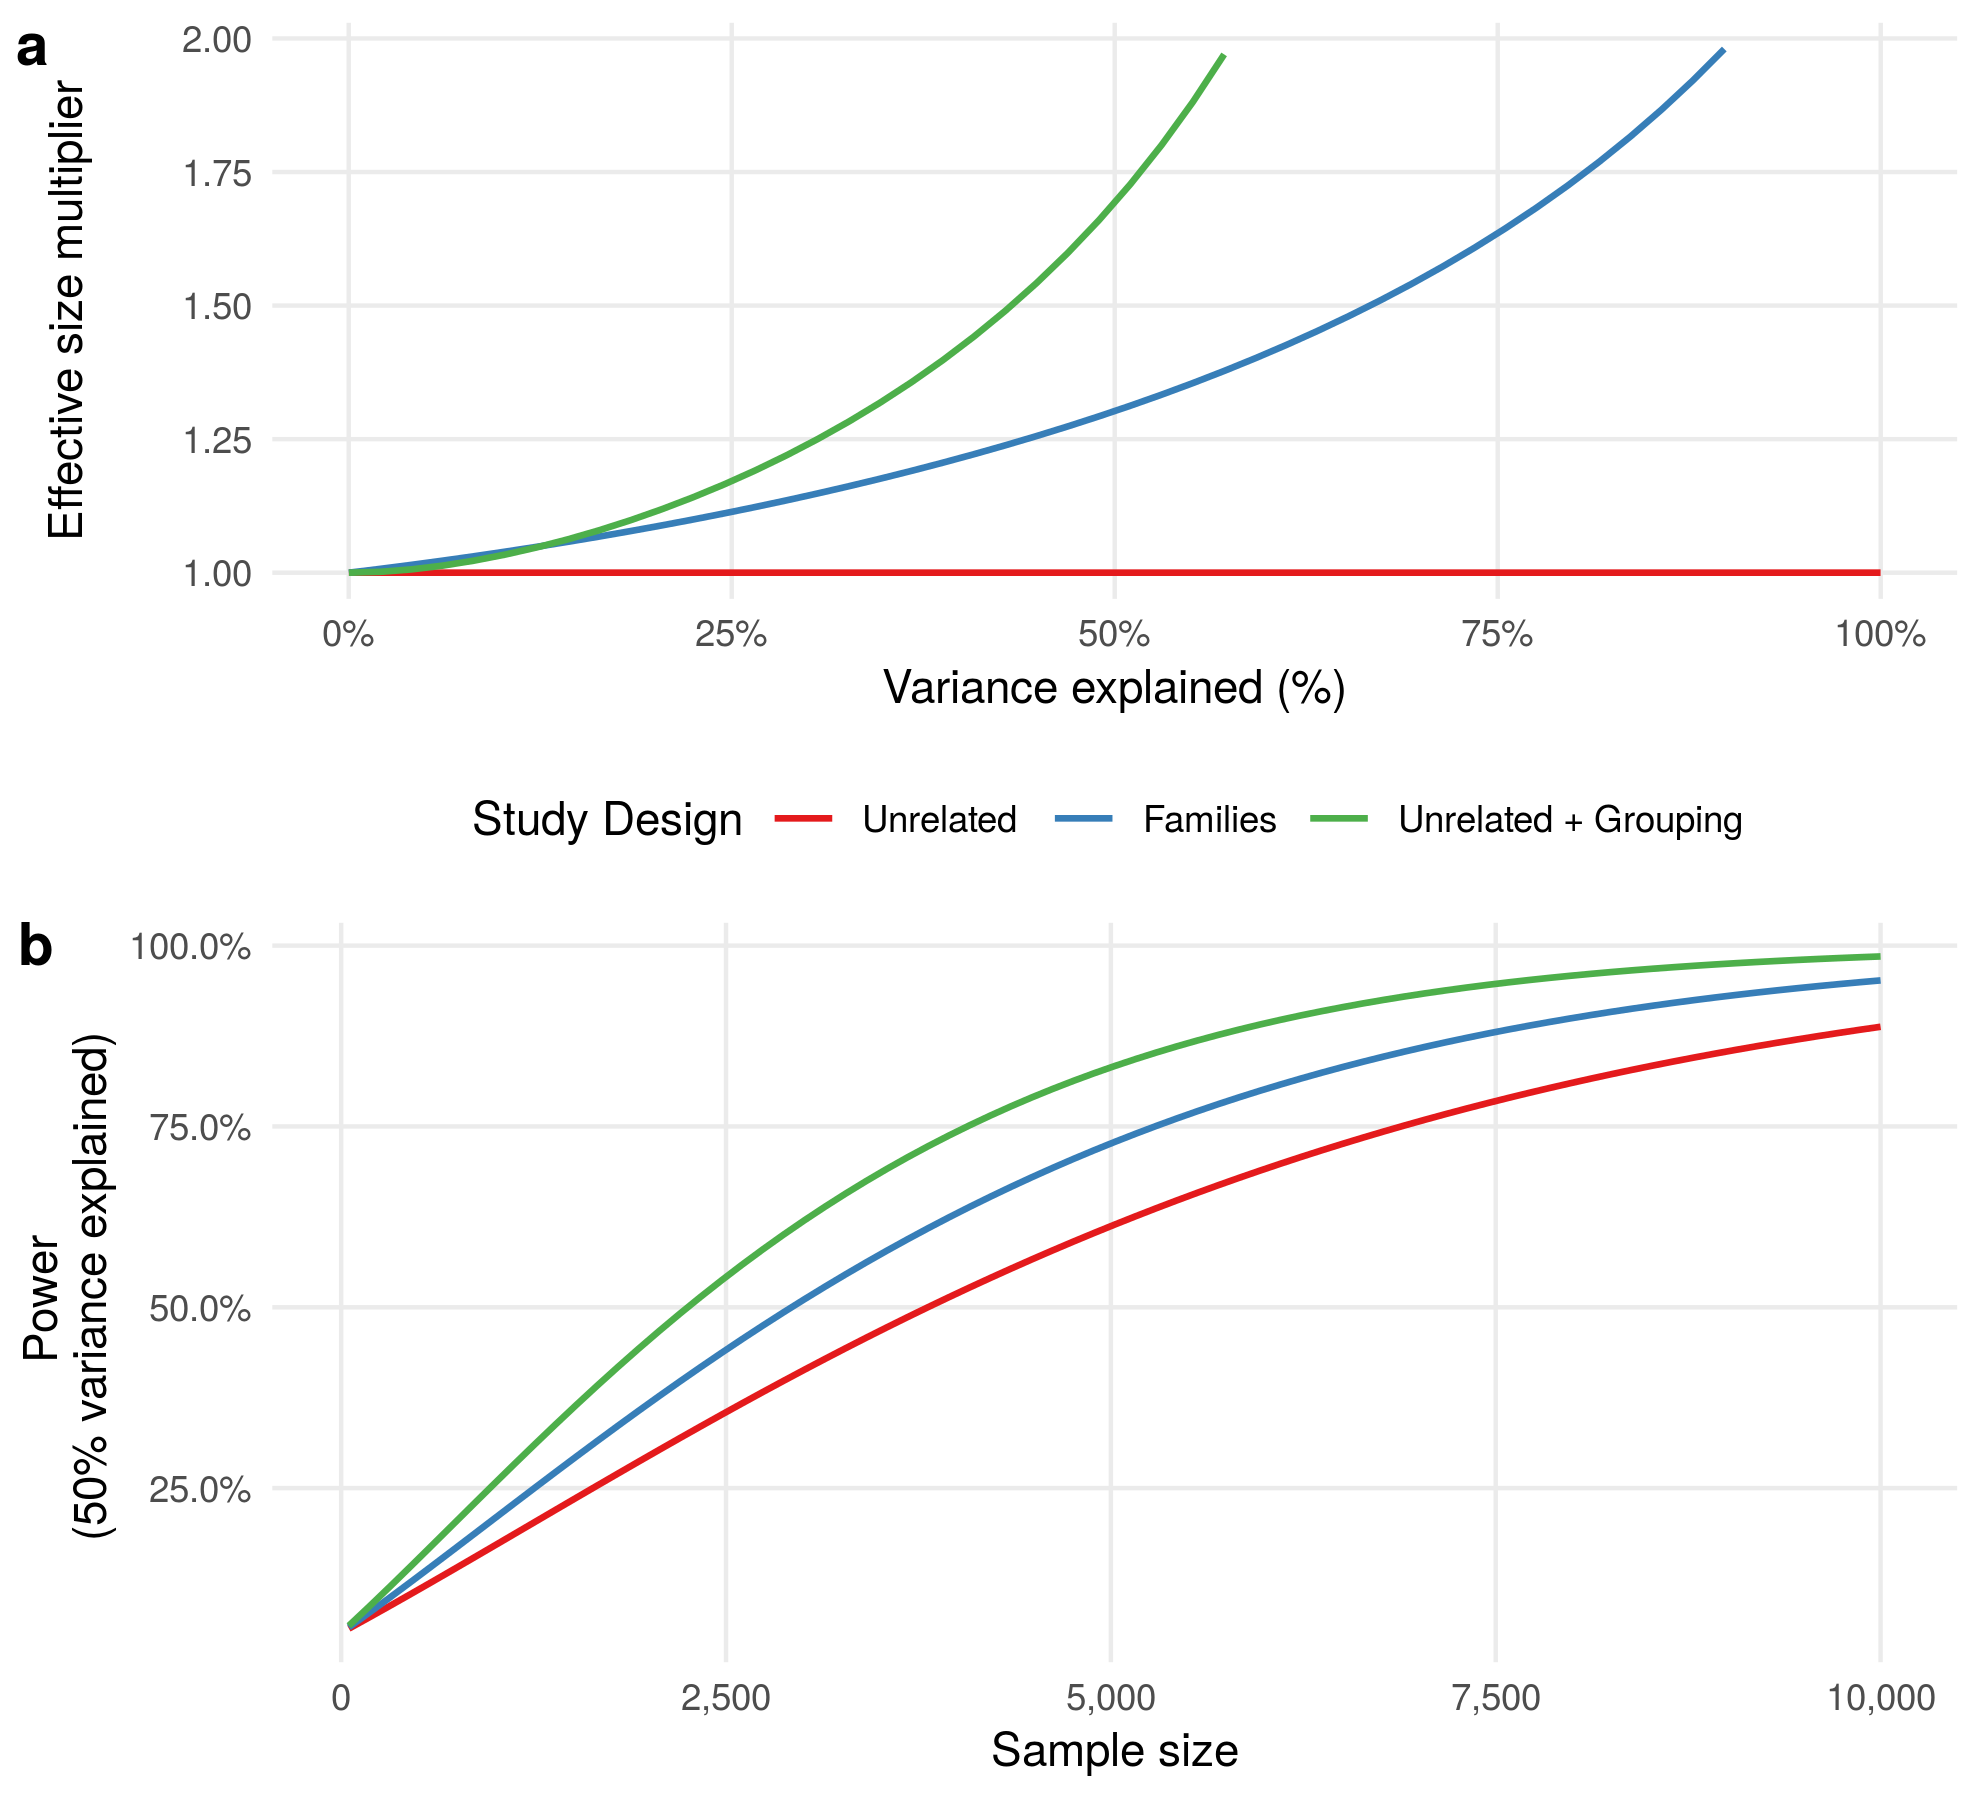
\includegraphics[width=0.75\linewidth]{figures/09-figure-power-interaction-expsib-two-panels} 

}

\caption{Comparison of study designs to detect
gene-environment interaction effect. The binary exposure is generated
such a way that siblings are exposed, while parents don't (the frequency
of exposure \(f = 3/5 = 0.6\)).}\label{fig:power-interaction}
\end{figure}






Ref \ref{fig:power-interaction}

\subsection{Implication in association
studies}\label{implication-in-association-studies}

\subsubsection{Effective sample size in post-GWAS
analyses}\label{effective-sample-size-in-post-gwas-analyses}

Many post-GWAS analyses, such as LDSC regresssion or meta-analysis, rely
on the sample size as an input parameter under assumption that summary
statistics come from a set of unrelated individuals under association
linear model. Though, tools that employ linear mixed models, for
example, BOLT-LMM, achieve the effective sample size (\(n_{eff}\))
larger than the true sample size (\(n\)) \citep{loh2018mixed}.

Gazal \emph{et al.} showed that the LDSC regression overestimates
per-variant heritability when using summary statistics from BOLT-LMM and
the true sample size (\(n\)) \citep{Gazal2017}. The authors proposed an
empirical solution to estimate the scaling factor or the effective size
multiplier: taking ratios of chi-squared statistics computed by BOLT-LMM
\emph{vs.} linear regression at genome-wide significant variants
\citep{loh2018mixed}. In our work, we derived an analytical form for the
effective size multiplier in Equations \eqref{eq:ncpg} and
\eqref{eq:ncpggrm}.

\subsubsection{Optimization of study
design}\label{optimization-of-study-design}

In genetic association and linkage studies performed in related
individuals grouped in families, selection of a family-based design that
achieves the most statistical power has been extensively studied
{[}ref{]}. For example, the multipoint linkage analysis was shown to
have greater power in extended pedigrees than in smaller pedigrees such
as sibships \citep{Almasy1998}.

\chapter{Supplementary Material}\label{supplementary-material}

\section{Propositions}\label{propositions}

\textbf{Quadratic form}: If \(\mathcal{X}\) is a vector of random
variables with mean \(\mu\) and (nonsingular) covariance matrix
\(\Sigma\), then the quadratic form \(\mathcal{X}^T A \mathcal{X}\) is a
scalar random variable:

\begin{equation}
E(\mathcal{X}^T A \mathcal{X}) = tr(A\Sigma) + \mu^T \Sigma \mu
\label{eq:quadform1}
\end{equation}

\begin{equation}
Var(\mathcal{X}^T A \mathcal{X}) = 2tr(A \Sigma A \Sigma) + 4\mu A \Sigma A \mu
\label{eq:quadform2}
\end{equation}

See \citep[Appendix 3, pp.~843]{Lynch1998} for more details.

\textbf{A linear transform of a random vector}: If \(B\) is a constant
matrix and \(\mathcal{X}\) is a vector of random variables with mean
\(\mu\) and covariance matrix \(\Sigma\), then \(B \mathcal{X}\) is a
vector of random variables:

\begin{equation}
E(B \mathcal{X}) = B E(\mathcal{X})
\label{eq:matvec1}
\end{equation}

\begin{equation}
Var(B \mathcal{X}) = B Var(\mathcal{X}) B^T
\label{eq:matvec2}
\end{equation}

The proof makes use of definitions of mean and variance.

\textbf{Eigen-value decompostion (EVD)}: If \(K\) is the covariane
matrix of size \(n \times n\), that means \(K\) is symmetric and
positive semi-definite. Furthemore, EVD of \(K\) is

\begin{equation}
K = Q D Q^T = Q D Q^{-1}
\label{eq:evdk}
\end{equation}

where \(Q\) is an \(n \times n\) orthogonal matrix of eigen-vectors and
\(D\) is a \(n \times n\) diagonal matirx of eigen-values
(\(\lambda_{K}^i\) with \(i\) from 1 to \(n\)).

EVD for the matrix inverse to \(K\) is

\begin{equation}
K^{-1} = Q D^{-1} Q^T
\label{eq:evdkinv}
\end{equation}

EVD for the matrix such as \(V = a K + b I\), where \(a\) and \(b\) are
scalars, \(I\) is the \(n \times n\) identity matrix, is

\begin{equation}
V = a K + b I = a Q D Q^T + b I = a Q D Q^T + b Q I Q^T = Q (a K + b I) Q^T
\label{eq:evdkinv}
\end{equation}

\textbf{Eigen-value decompostion (EVD) and the trace operator}: For the
covariance matrix \(K\) and the matrix \(V = a K + b I\), we have the
following serie of equation in relation to the trace operator.

\begin{equation}
\begin{split}
tr(K) & = \sum_{i=1}^{n}{\lambda_{K}^i} \\
tr(K^{-1}) & = \sum_{i=1}^{n}{(\lambda_{K}^i)^{-1}} \\
tr(V) = tr(a K + b I) & = \sum_{i=1}^{n}{(a \lambda_{K}^i + b)} \\
tr(V^{-1}) = tr((a K + b I)^{-1}) & = \sum_{i=1}^{n}{(a \lambda_{K}^i + b)^{-1}} \\
tr(V^{-1} K) = tr((a K + b I)^{-1} K) = tr((a I + b K^{-1})^{-1}) & = \sum_{i=1}^{n}{(a + b (\lambda_{K}^i)^{-1})^{-1}}
\end{split}
\label{eq:evdtr}
\end{equation}

In the last equation we used the following equality.

\begin{equation}
\begin{split}
V^{-1} K & = (a K + b I)^{-1} K = (a K + b I)^{-1} (K^{-1})^{-1} \\
 & = K^{-1} (a K + b I)^{-1} = (a I + b K^{-1})^{-1}
\end{split}
\label{eq:vinv}
\end{equation}

\section{Analytical derivations}\label{derivations}

To study the impact of relatedness among individuals on modeling a
continuous phenotype \(y\), we consider the following linear mixed
model:

\begin{equation}
  y = X \beta + \sum_{k=1}^{m}{r_k} + e
\label{eq:lmm}
\end{equation}

where \(n\) is the number of individuals, \(p\) is the number of
covariates or fixed effects, \(m\) is the number of structured random
effects apart from the residuals errors, \(y\) is a phenotype vector of
length \(n\), \(X\) is a matrix of covariates of size \(n \times p\),
\(\beta\) is a vector of fixed effects of length \(p\). The vectors of
random effects \(r_k\) and \(e\) are mutually uncorrelated and
multivariate normally distributed as \(\mathcal{N}(0, \sigma^2_k R_k)\)
and \(\mathcal{N}(0, \sigma^2_r I)\). The variance-covariance matrices
are parametrized with scalar parameters and constant matrices of size
\(n \times n\) that express relationships among \(n\) individuals. The
first \(m\) random effects \(r_k\) are referred here as structured,
whereas the last component \(e\) is simply the residual errors which are
independent and identically distributed.

Thus, the phenotype follows a multivariate normal distribution (MVN) and
Equation \eqref{eq:lmm} can be rewritten:

\begin{equation}
  y \sim \mathcal{N} (X \beta, V) = \mathcal{N} (X \beta, \sum_{k=1}^{m}{\sigma_k^2 R_k} + \sigma_r^2 I) 
\label{eq:mvn}
\end{equation}

We further consider several parameterizations of the model in Equation
\eqref{eq:mvn} that depend on (i) whether marginal genetic or
gene-environment interaction effect is under testing; (ii) whether
structured random effects are included or only the residual errors.
Consequently, the composition of fixed and random effects are updated
accordingly via the matrices \(X\) and \(V\), respectively.

\subsection{Testing marginal genetic effect in unrelated
individuals}\label{lmg}

We rewrite Equation \eqref{eq:mvn} as following:

\begin{equation}
  y \sim \mathcal{N} (X \beta, V) = \mathcal{N} (\mu x_0 + \beta_g x_g, \sigma_r^2 I) 
\label{eq:lmg}
\end{equation}

where \(x_0 = 1_n\) is a vector of \(n\) ones, \(\mu\) is a mean of the
phenotypic values, \(x_g\) is a vector of length of the genotypic
values, \(\beta_g\) is the effect size of the genotype.

The ordinary least squares (OLS) solution for fixed effects is the
following in the matrix form, \(\hat{\beta} = (X^T X)^{-1} X y\).
Further, the effect \(\beta_g\) can be estimated separately from the
mean effect \(\mu\) if vectors \(y\) and \(x_g\) are centered and, thus,
the two vectors are uncorrelated. Hence, the estimated effect is
expressed as
\(\hat{\beta_g} = \left(\tilde{x}_g^T \tilde{x}_g\right)^{-1} \tilde{x}_g \tilde{y}\),
where \(\tilde{x}_g\) and \(\tilde{y}\) are centered vectors \(x_g\) and
\(y\), respectively. The variance of the estimate is
\(var(\hat{\beta_g}) = \sigma_r^2 / (\tilde{x}_g^T \tilde{x}_g)\) and
the final expression is the following:

\begin{equation}
  \hat{\beta}_g  = \left(\tilde{x}_g^T \tilde{x}_g\right)^{-1} \tilde{x}_g^T \tilde{y} \sim \mathcal{N} (\beta_g, \sigma_r^2 / (\tilde{x}_g^T \tilde{x}_g))
\label{eq:betahatlmg}
\end{equation}

We next approximate the expression \(\tilde{x}_g^T \tilde{x}_g\) by
using the fact that that \(x_g\) is a realization of a vector of random
variables \(\mathcal{X_g}\), which is a genotype in \(n\) unrelated
individuals with a minor allele frequency \(p\). Consequently, we denote
\(\mathcal{X_g} \sim (\mu_g, \Sigma_g) = (p 1_n, \delta_g^2 I) = (p 1_n, 2 p (1-p) I)\)
and also \(\mathcal{\tilde{X}_g} \sim (0_n, \Sigma_g)\), where \(I\) is
the identity matrix of size \(n \times n\), \(1_n\) is a vector of \(n\)
ones and \(0_n\) is a vector of \(n\) zeros. Applying the proposition
for quadratic forms in Equation \eqref{eq:quadform2} for
\(\mathcal{\tilde{X}_g}\), we obtain the approximation:

\begin{equation}
\tilde{x}_g^T \tilde{x}_g \approx E(\mathcal{\tilde{X}_g}^T \mathcal{\tilde{X}_g}) = tr(\delta_g^2 I) = \delta_g^2 n = 2 p (1 - p) n
\label{eq:varbetahatlmg}
\end{equation}

The NCP parameter for testing the marginal genetic effect in unrelated
individuals is approximated as following:

\begin{equation}
NCP_{unrel} = \hat{\beta}_g^2 / var(\hat{\beta}_g) \approx \hat{\beta}_g^2 \delta_g^2 n / \sigma_r^2 = \hat{\beta}_g^2 2 p (1 - p) n / \sigma_r^2
\label{eq:ncplmg}
\end{equation}

If the the phenotype \(y\) is standardized, i.e. \(var(y) = 1\) and the
effect \(\beta_g\) is small, then we can further approximate
\(\sigma_r^2 \approx 1\) based on the following:

\begin{equation}
\begin{split}
\sigma^2_r & \approx \hat{\sigma}^2_r = \hat{e}^T \hat{e} / (n - 2) \\
& = (\tilde{y} - \hat{\beta}_g \tilde{x})^T (\tilde{y} - \hat{\beta}_g \tilde{x}) / (n - 2) \approx \tilde{y}^T \tilde{y} / (n - 2) \approx 1
\end{split}
\label{eq:sigma2r}
\end{equation}

Hence, we obtain the NCP estimation for the scaled phenotype:

\begin{equation}
NCP_{unrel} = \hat{\beta}_g^2 / var(\hat{\beta}_g) \approx \hat{\beta}_g^2 \delta_g^2 n  = \hat{\beta}_g^2 2 p (1 - p) n
\label{eq:ncplmg}
\end{equation}

\subsection{Testing marginal genetic effect in related
individuals}\label{lmmg}

We rewrite Equation \eqref{eq:mvn} as following:

\begin{equation}
  y \sim \mathcal{N} (X \beta, V) = \mathcal{N} (\mu x_0 + \beta_g x_g, \sum_{k=1}^{m}{\sigma_k^2 R_k} + \sigma_r^2 I) 
\label{eq:lmmg}
\end{equation}

The initial step in solving a linear mixed model is to estimate random
effects parameters (\(\sigma_k^2\) and \(\sigma_r^2\)) by maximum
likelihood (ML), restricted maximum likelihood (REML) or other
optimization technique \citep{Lynch1998}. Once the estimate of the
variance-covariance matrix is found,
\(\hat{V} = \sum{\hat{\sigma}_i^2 R_i} + \hat{\sigma}_r^2 I\), the
generalized least squares (GLS) solution for fixed effects is applied in
the following matrix form,
\(\hat{\beta} = \left(X^T \hat{V}^{-1} X\right)^{-1} X \hat{V}^{-1} y\).
This solution is obvious if both parts of Equation \eqref{eq:lmmg} are
multiplied by \(\hat{V}^{-0.5}\), thus removing the correlation
structure in the random part.

\begin{equation}
  \hat{V}^{-0.5} y \sim \mathcal{N} (\mu \hat{V}^{-0.5} x_0 + \beta_x \hat{V}^{-0.5} x , I)
\label{eq:lmmg2}
\end{equation}

The expression for the genetic effect estimate is obtained similarly to
Equation \eqref{eq:betahatlmg} and working with centered vectors:

\begin{equation}
  \hat{\beta}_g  = (\tilde{x}_g^T \hat{V}^{-1} \tilde{x}_g)^{-1} \tilde{x}_g^T \hat{V}^{-1} \tilde{y} \sim \mathcal{N} (\beta_g, 1 / (\tilde{x}_g^T \hat{V}^{-1} \tilde{x}_g))
\label{eq:betahatlmmg}
\end{equation}

We further again consider the quadratic form
\(\tilde{x}_g^T \hat{V}^{-1} \tilde{x}_g\) and use its mean for
approximation, as shown in Equation \eqref{eq:quadform2}. A vector \(x_g\)
of the genotypic values is a realization of a vector of random variables
\(\mathcal{X_g} \sim (\mu_g, \Sigma_g) = (p 1_n, \delta_g^2 K) = (p 1_n, 2 p (1 - p) K)\),
where \(p\) is a minor allele frequency of the genotype and \(K\) is the
kinship matrix of size \(n \times n\). We also introduce a centered
vector of random variables \(\mathcal{X_g} \sim (0_n, \Sigma_g)\).

The matrix \(K\) expresses the genetic relatedness among \(n\)
individuals and it is the identity matrix \(I\) for genetically
unrelated individuals. The derivation presented here are appropriate for
any form of the matrix \(K\).

Treating the matrix \(\hat{V}^{-1}\) as a (constant) transformation
matrix \(A\) in Equation \eqref{eq:quadform2} for quadratic forms gives us
the approximation:

\begin{equation}
\tilde{x}_g^T \hat{V}^{-1} \tilde{x}_g \approx E(\mathcal{\tilde{X}_g}^T \hat{V}^{-1} \mathcal{\tilde{X}_g}) = tr(\hat{V}^{-1} \Sigma_g) = \delta_g^2 tr(\hat{V}^{-1} K) = 2 p (1 - p) tr(\hat{V}^{-1} K)
\label{eq:varbetahatlmmg}
\end{equation}

The NCP parameter for testing the marginal genetic effect in related
individuals is approximated as following:

\begin{equation}
\begin{split}
NCP_{rel} & = \hat{\beta}_g^2 / var(\hat{\beta}_g) \approx \hat{\beta}_g^2 tr(\hat{V}^{-1} \Sigma_g) \\
 & = \hat{\beta}_g^2 \delta_g^2 tr(\hat{V}^{-1} K) = \hat{\beta}_g^2 2 p (1 - p) tr(\hat{V}^{-1} K)
\end{split}
\label{eq:ncplmg}
\end{equation}

\subsection{Effective size multiplier for testing marginal genetic
effect}\label{trfg}

We joint results from the previous two sections \ref{lmg} and \ref{lmmg}
to derive the formula for ratio between \(NCP_{rel}\) and
\(NCP_{unrel}\), as referred herein the effective size multiplier.

\begin{equation}
NCP_{rel} / NCP_{unrel} =  tr(\hat{V}^{-1} K) / (n / \sigma^2_r)
\label{eq:ncpratio}
\end{equation}

If the variance of the phenotype \(y\) is standardized to 1 and the
variance captured by the genotype is small, then we can approximate
\(\sigma_r^2 \approx 1\) in Equation \eqref{eq:ncplmg} and further obtain:

\begin{equation}
NCP_{rel} / NCP_{unrel} = tr(\hat{V}^{-1} K) / n
\label{eq:ncpratiosc}
\end{equation}

The variance components in \(\hat{V}\) are then considered as the
proportions, since the variance of the phenotype \(y\) is standardized
to 1.

\subsection{Testing gene-environment interaction effect in unrelated
individuals}\label{lmge}

We rewrite Equation \eqref{eq:mvn} as following:

\begin{equation}
  y \sim \mathcal{N} (X \beta, V) = \mathcal{N} (\mu x_0 + \beta_g x_g + \beta_e x_e + \beta_{ge} x_{ge}, \sigma_r^2 I) 
\label{eq:lmge}
\end{equation}

where \(x_0 = 1_n\) is a vector of \(n\) ones, \(\mu\) is a mean of the
phenotypic values, \(x_g\) is a genotype vector of length \(n\),
\(\beta_g\) is the effect size of the genotype, \(x_e\) is a environment
exposure vector of length \(n\), \(\beta_e\) is the effect size of the
environment exposure, \(x_{ge}\) is a vector of length \(n\) of
gene-environment interaction, \(\beta_{ge}\) is the interaction effect
size.

The coding scheme of the genotypic and environmental variables to study
gene-environment interaction under the standard linear model has been
reviewed elsewhere \citep{Aschard2016}. Here, we work with centered
variables \(\tilde{x}_g\) and \(\tilde{x}_e\), and define the
interaction variable \(\tilde{x}_{ge}\) by (i) element-wise
multiplication of the two variables denoted as
\(\ddot{x}_{ge} = \tilde{x}_g \circ \tilde{x}_e\), (ii) centering the
resulted product \(\ddot{x}_{ge}\). Hence, the effect size for each
variable (columns in \(X\)) can be estimated independently from the
other variables under assumption that the two random variables of
genotype and environmental exposure are independent \citep[Appendix
C]{Aschard2016}. Of a note, different coding schemes give different
estimates of effect sizes, but the test statistic for gene-environment
interaction is the same \citep[Appendix B]{Aschard2016}.

Therefore, the estimate of interest \(\hat{\beta}_{ge}\) has the
following distribution:

\begin{equation}
  \hat{\beta}_{ge}  = \left(\tilde{x}_{ge}^T \tilde{x}_{ge}\right)^{-1} \tilde{x}_{ge}^T \tilde{y} \sim \mathcal{N} (\beta_{ge}, \sigma_r^2 / (\tilde{x}_{ge}^T \tilde{x}_{ge}))
\label{eq:betahatlmge}
\end{equation}

To further approximate the quantity \(\tilde{x}_{ge}^T \tilde{x}_{ge}\),
we need to work with two random variables. The first one is a vector of
random variables
\(\mathcal{\tilde{X}_g} \sim (0_n, \Sigma_g) = (0_n, \delta_g^2 I) = (0_n, 2 p (1-p) I)\),
which we previously described. The second is a vector of random
variables
\(\mathcal{\tilde{X}}_{ge} = \tilde{x}_e \circ \mathcal{\tilde{X}}_g = E \mathcal{\tilde{X}}_g\),
which is a transformed variable of \(\mathcal{\tilde{X}_g}\) with the
transformation matrix \(E = \mathrm{diag}(\tilde{x}_e)\), defined as a
diagonal matrix with values equal to those observed in the environmental
exposure. The operator \(\circ\) denotes the element-wise multiplication
(the Hadamard product).

We also consider a simple case for the environmental exposure when it is
binary and the observed frequency of exposure is \(f\). Then the values
on diagonal of the matrix \(E\) are equal \(-f\) and \(1 - f\), and we
denote this matrix as \(E_b\).

We further give an example of the matrix \(E_b\) for 5 individuals under
study with the first two unexposed and the last three exposed to the
environment, i.e. \(f = 0.6\).

\begin{equation*} 
E_b = 
\left(\begin{array}{ccccc}
0 & 0 & 0 & 0 & 0\\
0 & 0 & 0 & 0 & 0\\
0 & 0 & 1 & 0 & 0\\
0 & 0 & 0 & 1 & 0\\
0 & 0 & 0 & 0 & 1\\
\end{array}\right)
- 
\left(\begin{array}{c}
0.6 \\
0.6 \\
0.6 \\
0.6 \\
0.6 \\
\end{array}\right)
= 
\left(\begin{array}{ccccc}
-0.6 & 0 & 0 & 0 & 0\\
0 & -0.6 & 0 & 0 & 0\\
0 & 0 & 0.4 & 0 & 0\\
0 & 0 & 0 & 0.4 & 0\\
0 & 0 & 0 & 0 & 0.4\\
\end{array}\right)
\end{equation*}

We first need to derive the variance of the random variable
\(\mathcal{\tilde{X}}_{ge}\). We obtain from Equation \eqref{eq:matvec2}:

\begin{equation}
\begin{split}
\mathrm{Var}(\mathcal{\tilde{X}}_{ge}) & = \mathrm{Var}(E \mathcal{\tilde{X}}_g) = E \mathrm{Var}(\mathcal{\tilde{X}}_g) E^T \\
 & = E (\delta_g^2 I) E^T = \delta_g^2 E E^T = \delta_g^2 E^2 
\end{split}
\label{eq:xgevar}
\end{equation}

Applying the results for quadratic forms in Equation \eqref{eq:quadform2}
gives us the approximation:

\begin{equation}
\tilde{x}_{ge}^T \tilde{x}_{ge} \approx E(\mathcal{\tilde{X}}_{ge}^T \mathcal{\tilde{X}}_{ge}) = tr(\delta_g^2 E^2) = \delta_g^2 tr(E^2) = 2 p (1 - p) tr(E^2)
\label{eq:varbetahatlmg}
\end{equation}

When the exposure is binary, we can simplify this quantity using the
following equality \(tr(E_b) = f (1 - f) n\):

\begin{equation}
\tilde{x}_{ge}^T \tilde{x}_{ge} \approx \delta_g^2 f (1 - f) n = 2 p (1 - p) f (1 - f) n
\label{eq:varbetahatlmgbin}
\end{equation}

Next, the NCP parameter for testing the gene-environment interaction
effect in unrelated individuals is approximated as following:

\begin{equation}
NCP_{unrel + int} = \hat{\beta}_{ge}^2 / var(\hat{\beta}_{ge}) \approx \hat{\beta}_{ge}^2 \delta_g^2 tr(E^2) / \sigma_r^2 = \hat{\beta}_{ge}^2 2 p (1 - p) tr(E^2) / \sigma_r^2
\label{eq:ncplmge}
\end{equation}

When the exposure is binary:

\begin{equation}
NCP_{unrel + int} = \hat{\beta}_{ge}^2 / var(\hat{\beta}_{ge}) \approx \hat{\beta}_{ge}^2 \delta_g^2 tr(E_b^2) / \sigma_r^2 = \hat{\beta}_{ge}^2 2 p (1 - p) f (1 - f) n / \sigma_r^2
\label{eq:ncplmgebin}
\end{equation}

Additionally, we approximate \(\sigma_r^2 \approx 1\) if the the
phenotype \(y\) is standardized and the variance captured by all
genetic, environmental and interaction effects is small.

\subsection{Testing gene-environment interaction effect in related
individuals}\label{lmmge}

We rewrite Equation \eqref{eq:mvn} as following:

\begin{equation}
  y \sim \mathcal{N} (X \beta, V) = \mathcal{N} (\mu x_0 + \beta_g x_g + \beta_e x_e + \beta_{ge} x_{ge}, \sum_{k=1}^{m}{\sigma_k^2 R_k} + \sigma_r^2 I) 
\label{eq:lmmge}
\end{equation}

As in the previous derivation in Section \ref{lmge}, we apply the same
coding scheme for genetic, environmental and gene-environmental
interaction variables, \(\tilde{x}_g\), \(\tilde{x}_e\) and
\(\tilde{x}_{ge}\), respectively. As in the previous Section \ref{lmmg},
we derive the distribution of \(\hat{\beta}_{ge}\) conditionally on the
estimate of the variance-covariance matrix
\(\hat{V} = \sum{\hat{\sigma}_i^2 R_i} + \hat{\sigma}_r^2 I\):

\begin{equation}
  \hat{\beta}_{ge}  = \left(\tilde{x}_{ge}^T \hat{V}^{-1} \tilde{x}_{ge}\right)^{-1} \tilde{x}_{ge}^T \hat{V}^{-1} \tilde{y} \sim \mathcal{N} (\beta_{ge}, 1 / (\tilde{x}_{ge}^T \hat{V}^{-1} \tilde{x}_{ge}))
\label{eq:betahatlmmge}
\end{equation}

Also as in the previous Section \ref{lmmg}, we consider the two random
vectors,
\(\mathcal{\tilde{X}_g} \sim (0_n, \Sigma_g) = (0_n, \delta_g^2 K) = (0_n, 2 p (1-p) K)\),
and
\(\mathcal{\tilde{X}}_{ge} = \tilde{x}_e \circ \mathcal{\tilde{X}}_g = E \mathcal{\tilde{X}}_g\).
The later is a transformed variable of \(\mathcal{\tilde{X}_g}\) with
the transformation matrix \(E = \mathrm{diag}(\tilde{x}_e)\),

In addition, we introduce a matrix \(D\), which value at row \(i\) and
column \(j\) is equal to the product of two diagonal entries \(i\) and
\(j\) of \(E\), i.e. \(D_{i,j} = E_{i,i} E_{j,j}\). The use of this
matrix \(D\) is explained below.

When the environmental exposure is binary with the exposure frequency
\(f\), we denote the matrix \(E\) as \(E_b\) and the matrix \(D\) as
\(D_b\). The values on diagonal of \(E_b\) are either \(f\) or
\(1 - f\), while the values of \(D_b\) are either \(f^2\), \((1 - f)^2\)
or \(f (1 - f)\).

We derive the variance of the random variable
\(\mathcal{\tilde{X}}_{ge}\) using proposition in Equation
\eqref{eq:matvec2}:

\begin{equation}
\begin{split}
\mathrm{Var}(\mathcal{\tilde{X}}_{ge}) & = \mathrm{Var}(E \mathcal{\tilde{X}}_g) = E \mathrm{Var}(\mathcal{\tilde{X}}_g) E^T = E \Sigma_g E^T \\ 
 & = \delta_g^2 E K E^T = \delta_g^2 D \circ K = \delta_g^2 K_{D}
\end{split}
\label{eq:xgevar2}
\end{equation}

In the second part of derivation, we again used the fact that the matrix
\(E\) is diagonal; that means the expression \(E A E^T\) for a given
matrix A can be rewritten as \(D \circ A\), where the \(D\) was defined
before and the operator \(\circ\) denotes the element-wise
multiplication (the Hadamard product).

In Equation \eqref{eq:xgevar2} we introduced a special kinship matrix
\(K_{D}\) ``masked'' by the environmental exposure though the matrix
\(D\) defined above.

\begin{equation}
\begin{split}
K_{D} =  D \circ K
\end{split}
\label{eq:kd}
\end{equation}

We note that the \(K_{D}\) matrix becomes the \(E^2\) matrix in the
previous section \ref{lmge} when \(K = I\), i.e.~the case of unrelated
individuals.

For an illustration example, we show how the matrices \(E_b\), \(D_b\),
\(K\) and \(K_{D}\) look like for 5 individuals with the first two
unexposed and the last three exposed to the environment, i.e.
\(f = 0.6\). The five individuals represent a nuclear family of two
parents and three children.

\begin{equation*} 
E_b = 
\left(\begin{array}{ccccc}
-0.6 & 0 & 0 & 0 & 0\\
0 & -0.6 & 0 & 0 & 0\\
0 & 0 & 0.4 & 0 & 0\\
0 & 0 & 0 & 0.4 & 0\\
0 & 0 & 0 & 0 & 0.4\\
\end{array}\right)
\end{equation*}

\begin{equation*} 
D_b = 
\left(\begin{array}{ccccc}
-0.36 & -0.36 & -0.24 & -0.24 & -0.24\\
-0.36 & -0.36 & -0.24 & -0.24 & -0.24\\
-0.24 & -0.24 & 0.16 & 0.16 & 0.16\\
-0.24 & -0.24 & 0.16 & 0.16 & 0.16\\
-0.24 & -0.24 & 0.16 & 0.16 & 0.16\\
\end{array}\right)
\end{equation*}

\begin{equation*} 
K = 
\left(\begin{array}{ccccc}
1 & 0 & 0.5 & 0.5 & 0.5\\
0 & 1 & 0.5 & 0.5 & 0.5\\
0.5 & 0.5 & 1 & 0.5 & 0.5\\
0.5 & 0.5 & 0.5 & 1 & 0.5\\
0.5 & 0.5 & 0.5 & 0.5 & 1\\
\end{array}\right)
\end{equation*}

\begin{equation*} 
K_{D_b} = 
\left(\begin{array}{ccccc}
-0.36 & 0 & -0.12 & -0.12 & -0.12\\
0 & -0.36 & -0.12 & -0.12 & -0.12\\
-0.12 & -0.12 & 0.16 & 0.08 & 0.08\\
-0.12 & -0.12 & 0.08 & 0.16 & 0.08\\
-0.12 & -0.12 & 0.08 & 0.08 & 0.16\\
\end{array}\right)
\end{equation*}

Further applying the proposition for quadratic forms in Equation
\eqref{eq:quadform2} gives us the approximation:

\begin{equation}
\begin{split}
\tilde{x}_{ge}^T \hat{V}^{-1} \tilde{x}_{ge} & \approx E(\mathcal{\tilde{X}}_{ge}^T \hat{V}^{-1} \mathcal{\tilde{X}}_{ge}) = tr(\hat{V}^{-1} \delta_g^2 K_{D}) \\
& = \delta_g^2 tr(\hat{V}^{-1} K_{D}) = 2 p (1 - p) tr(\hat{V}^{-1} K_{D})
\end{split}
\label{eq:varbetahatlmmge}
\end{equation}

The NCP parameter for testing the gene-environment interaction effect in
related individuals is approximated as following:

\begin{equation}
NCP_{rel + int} = \hat{\beta}_{ge}^2 / var(\hat{\beta}_{ge}) \approx \hat{\beta}_{ge}^2 \delta_g^2 tr(\hat{V}^{-1} K_{D}) = \hat{\beta}_{ge}^2 2 p (1 - p) tr(\hat{V}^{-1} K_{D})
\label{eq:ncplmmge}
\end{equation}

\subsection{Effective size multiplier for testing marginal
gene-environment interaction effect}\label{trfge}

We joint results from the previous two sections \ref{lmge} and
\ref{lmmge} and present the formula for ratio between \(NCP_{rel+int}\)
and \(NCP_{unrel+int}\), as referred herein the effective size
multiplier.

\begin{equation}
NCP_{rel + int} / NCP_{unrel + int} = tr(\hat{V}^{-1} K_{D}) / (tr(E^2) / \sigma^2_r)
\label{eq:ncpratioge}
\end{equation}

If the variance of the phenotype \(y\) is standardized to 1 and the
variance captured by fixed effects is small, then we can approximate
\(\sigma_r^2 \approx 1\) in Equation \eqref{eq:ncplmge} and further
obtain:

\begin{equation}
NCP_{rel + int} / NCP_{unrel + int} = tr(\hat{V}^{-1} K_{D}) / tr(E^2)
\label{eq:ncpratiogesc}
\end{equation}

The variance components in \(\hat{V}\) are then considered as the
proportions, since the variance of the phenotype \(y\) is standardized
to 1.

\section{Simulations}\label{simulations}

\subsection{Unrelated: marginal genetic
effect}\label{unrelated-marginal-genetic-effect}

\begin{center}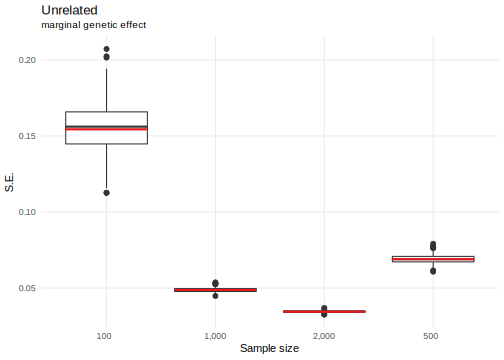
\includegraphics[width=1\linewidth]{gxefam_files/figure-latex/se_unrel_marginal-1} \end{center}

\subsection{Families: marginal genetic
effect}\label{families-marginal-genetic-effect}

\begin{center}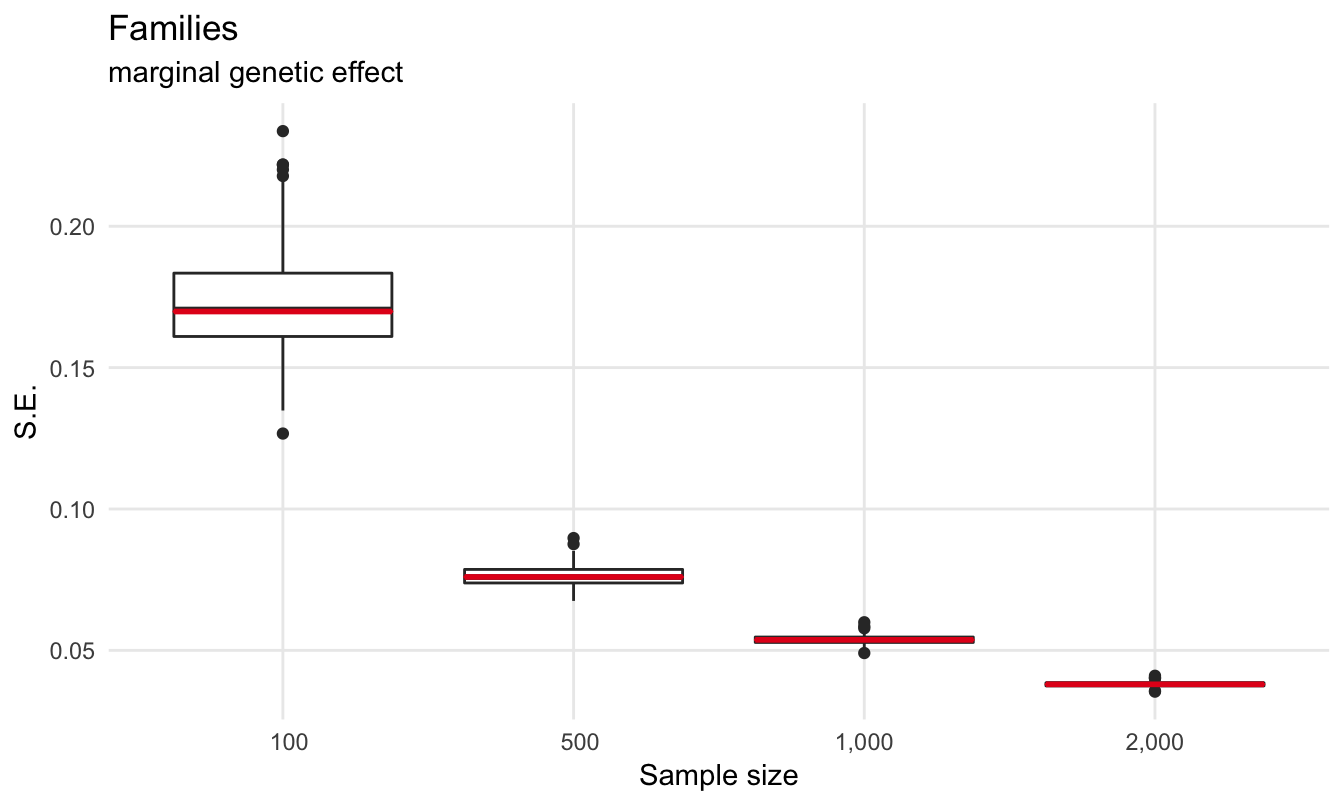
\includegraphics[width=1\linewidth]{gxefam_files/figure-latex/se_fam_marginal-1} \end{center}

\begin{tabular}{l|r}
\hline
Sample Size & Trace Factor\\
\hline
100 & 0.8253\\
\hline
500 & 0.8253\\
\hline
1,000 & 0.8253\\
\hline
2,000 & 0.8253\\
\hline
\end{tabular}

\subsection{Unrelated: interaction
effect}\label{unrelated-interaction-effect}

\begin{center}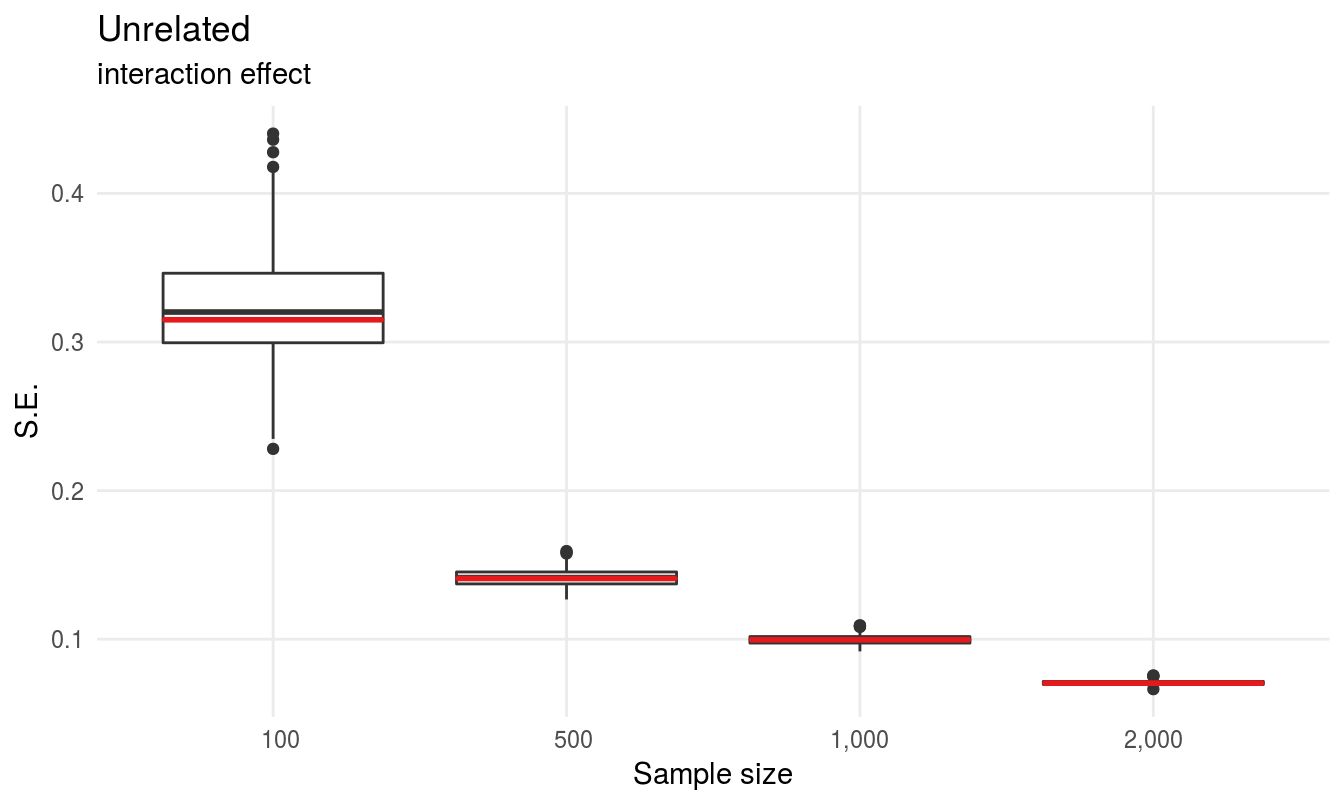
\includegraphics[width=1\linewidth]{gxefam_files/figure-latex/se_unrel_int-1} \end{center}

\subsection{Familes (two genetic components): interaction
effect}\label{familes-two-genetic-components-interaction-effect}

\begin{center}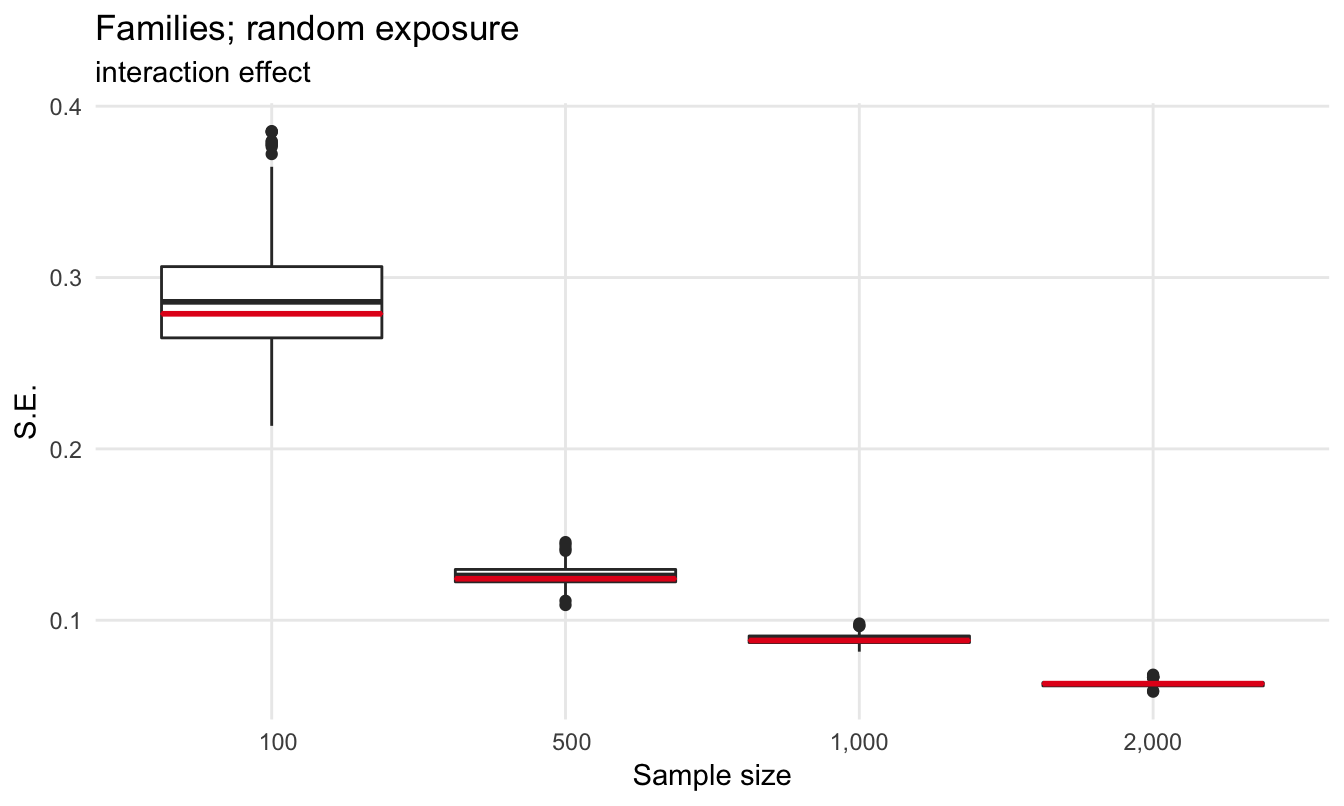
\includegraphics[width=1\linewidth]{gxefam_files/figure-latex/se_fam_int-1} \end{center}

\begin{tabular}{l|r}
\hline
Sample Size & Trace Factor\\
\hline
100 & 1.1921\\
\hline
500 & 1.2219\\
\hline
1,000 & 1.2333\\
\hline
2,000 & 1.2598\\
\hline
\end{tabular}

\subsection{Familes (one genetic component): interaction
effect}\label{familes-one-genetic-component-interaction-effect}

\begin{center}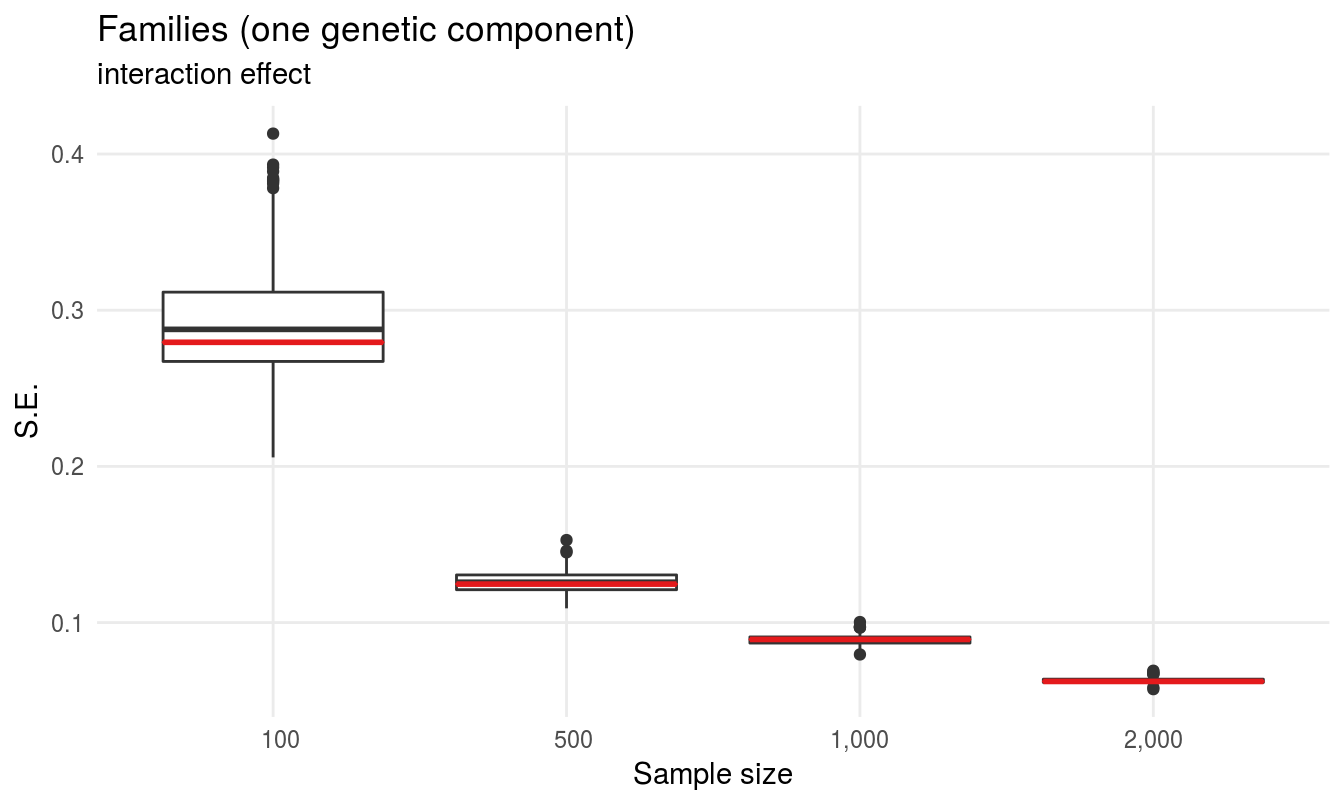
\includegraphics[width=1\linewidth]{gxefam_files/figure-latex/se_fam_int1-1} \end{center}

\begin{tabular}{l|r}
\hline
Sample Size & Trace Factor\\
\hline
100 & 1.2702\\
\hline
500 & 1.2773\\
\hline
1,000 & 1.2463\\
\hline
2,000 & 1.2775\\
\hline
\end{tabular}

\section{Supplementary Figures}\label{supplementary-figures}

\begin{figure}

{\centering 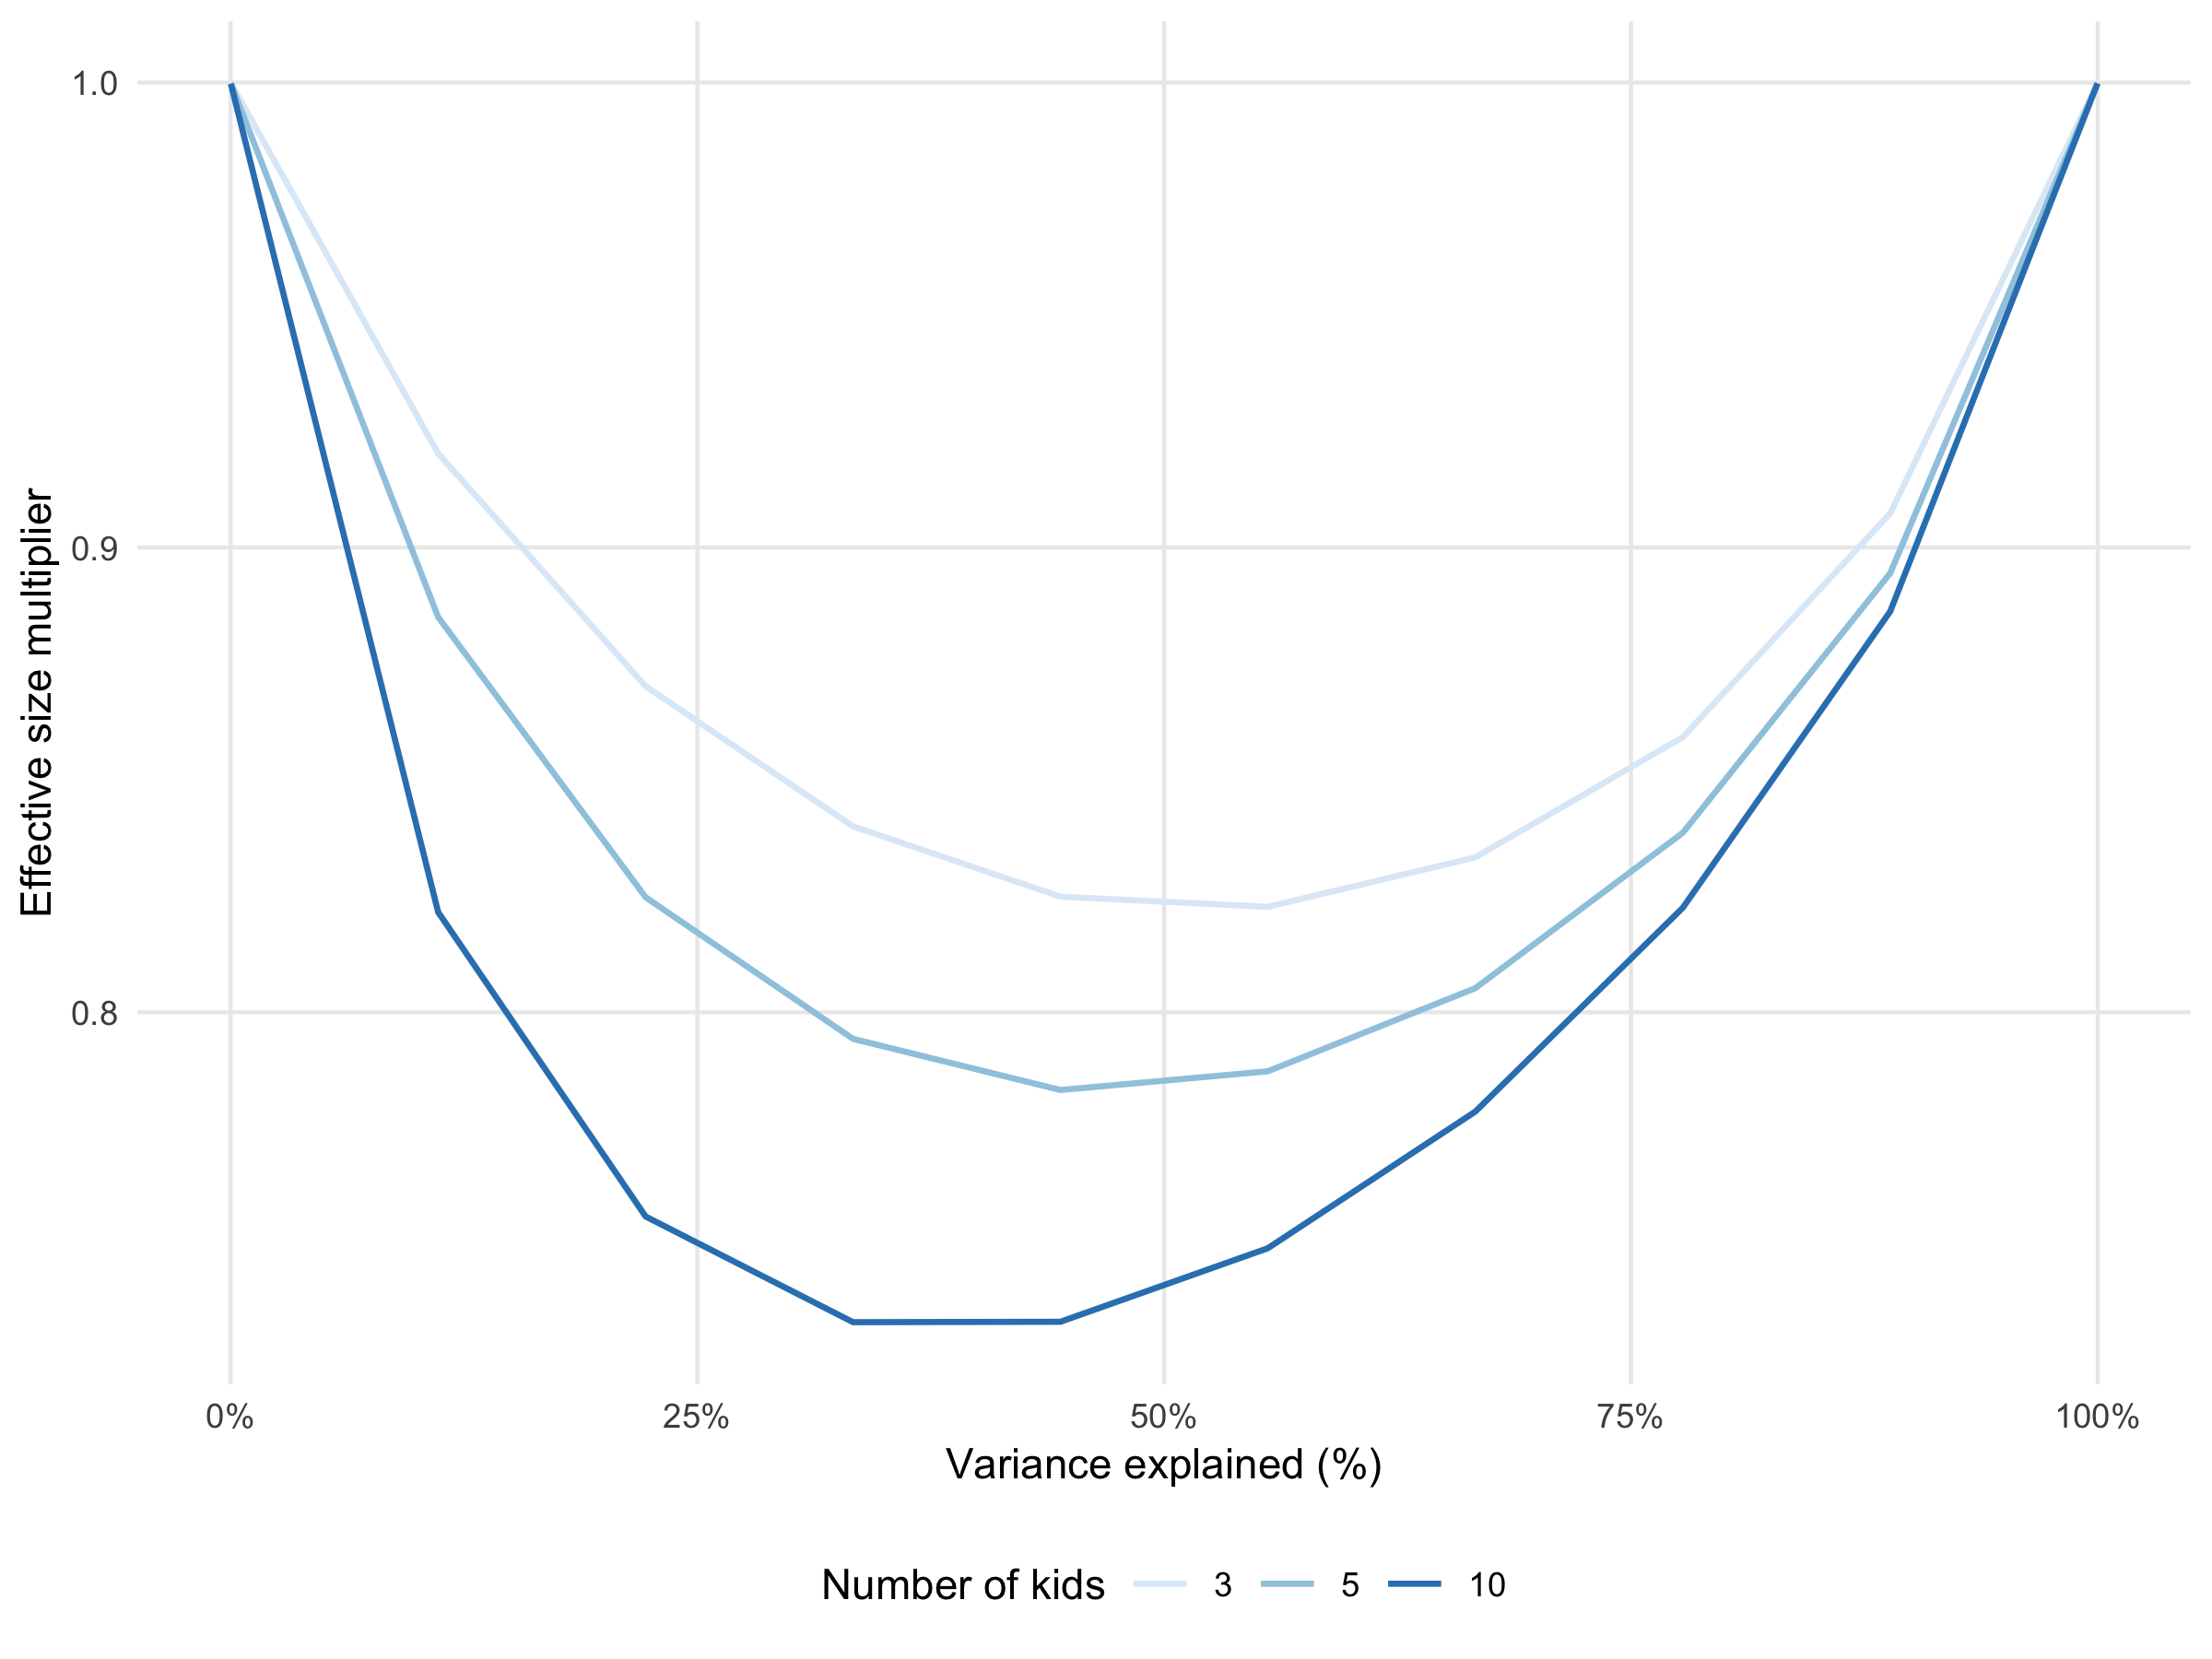
\includegraphics[width=1\linewidth]{figures/05-figure-sup-power-marginal-kids} 

}

\caption{Influence of family structure to detect
marginal genetic effect.}\label{fig:power-marginal-kids}
\end{figure}




\begin{figure}

{\centering 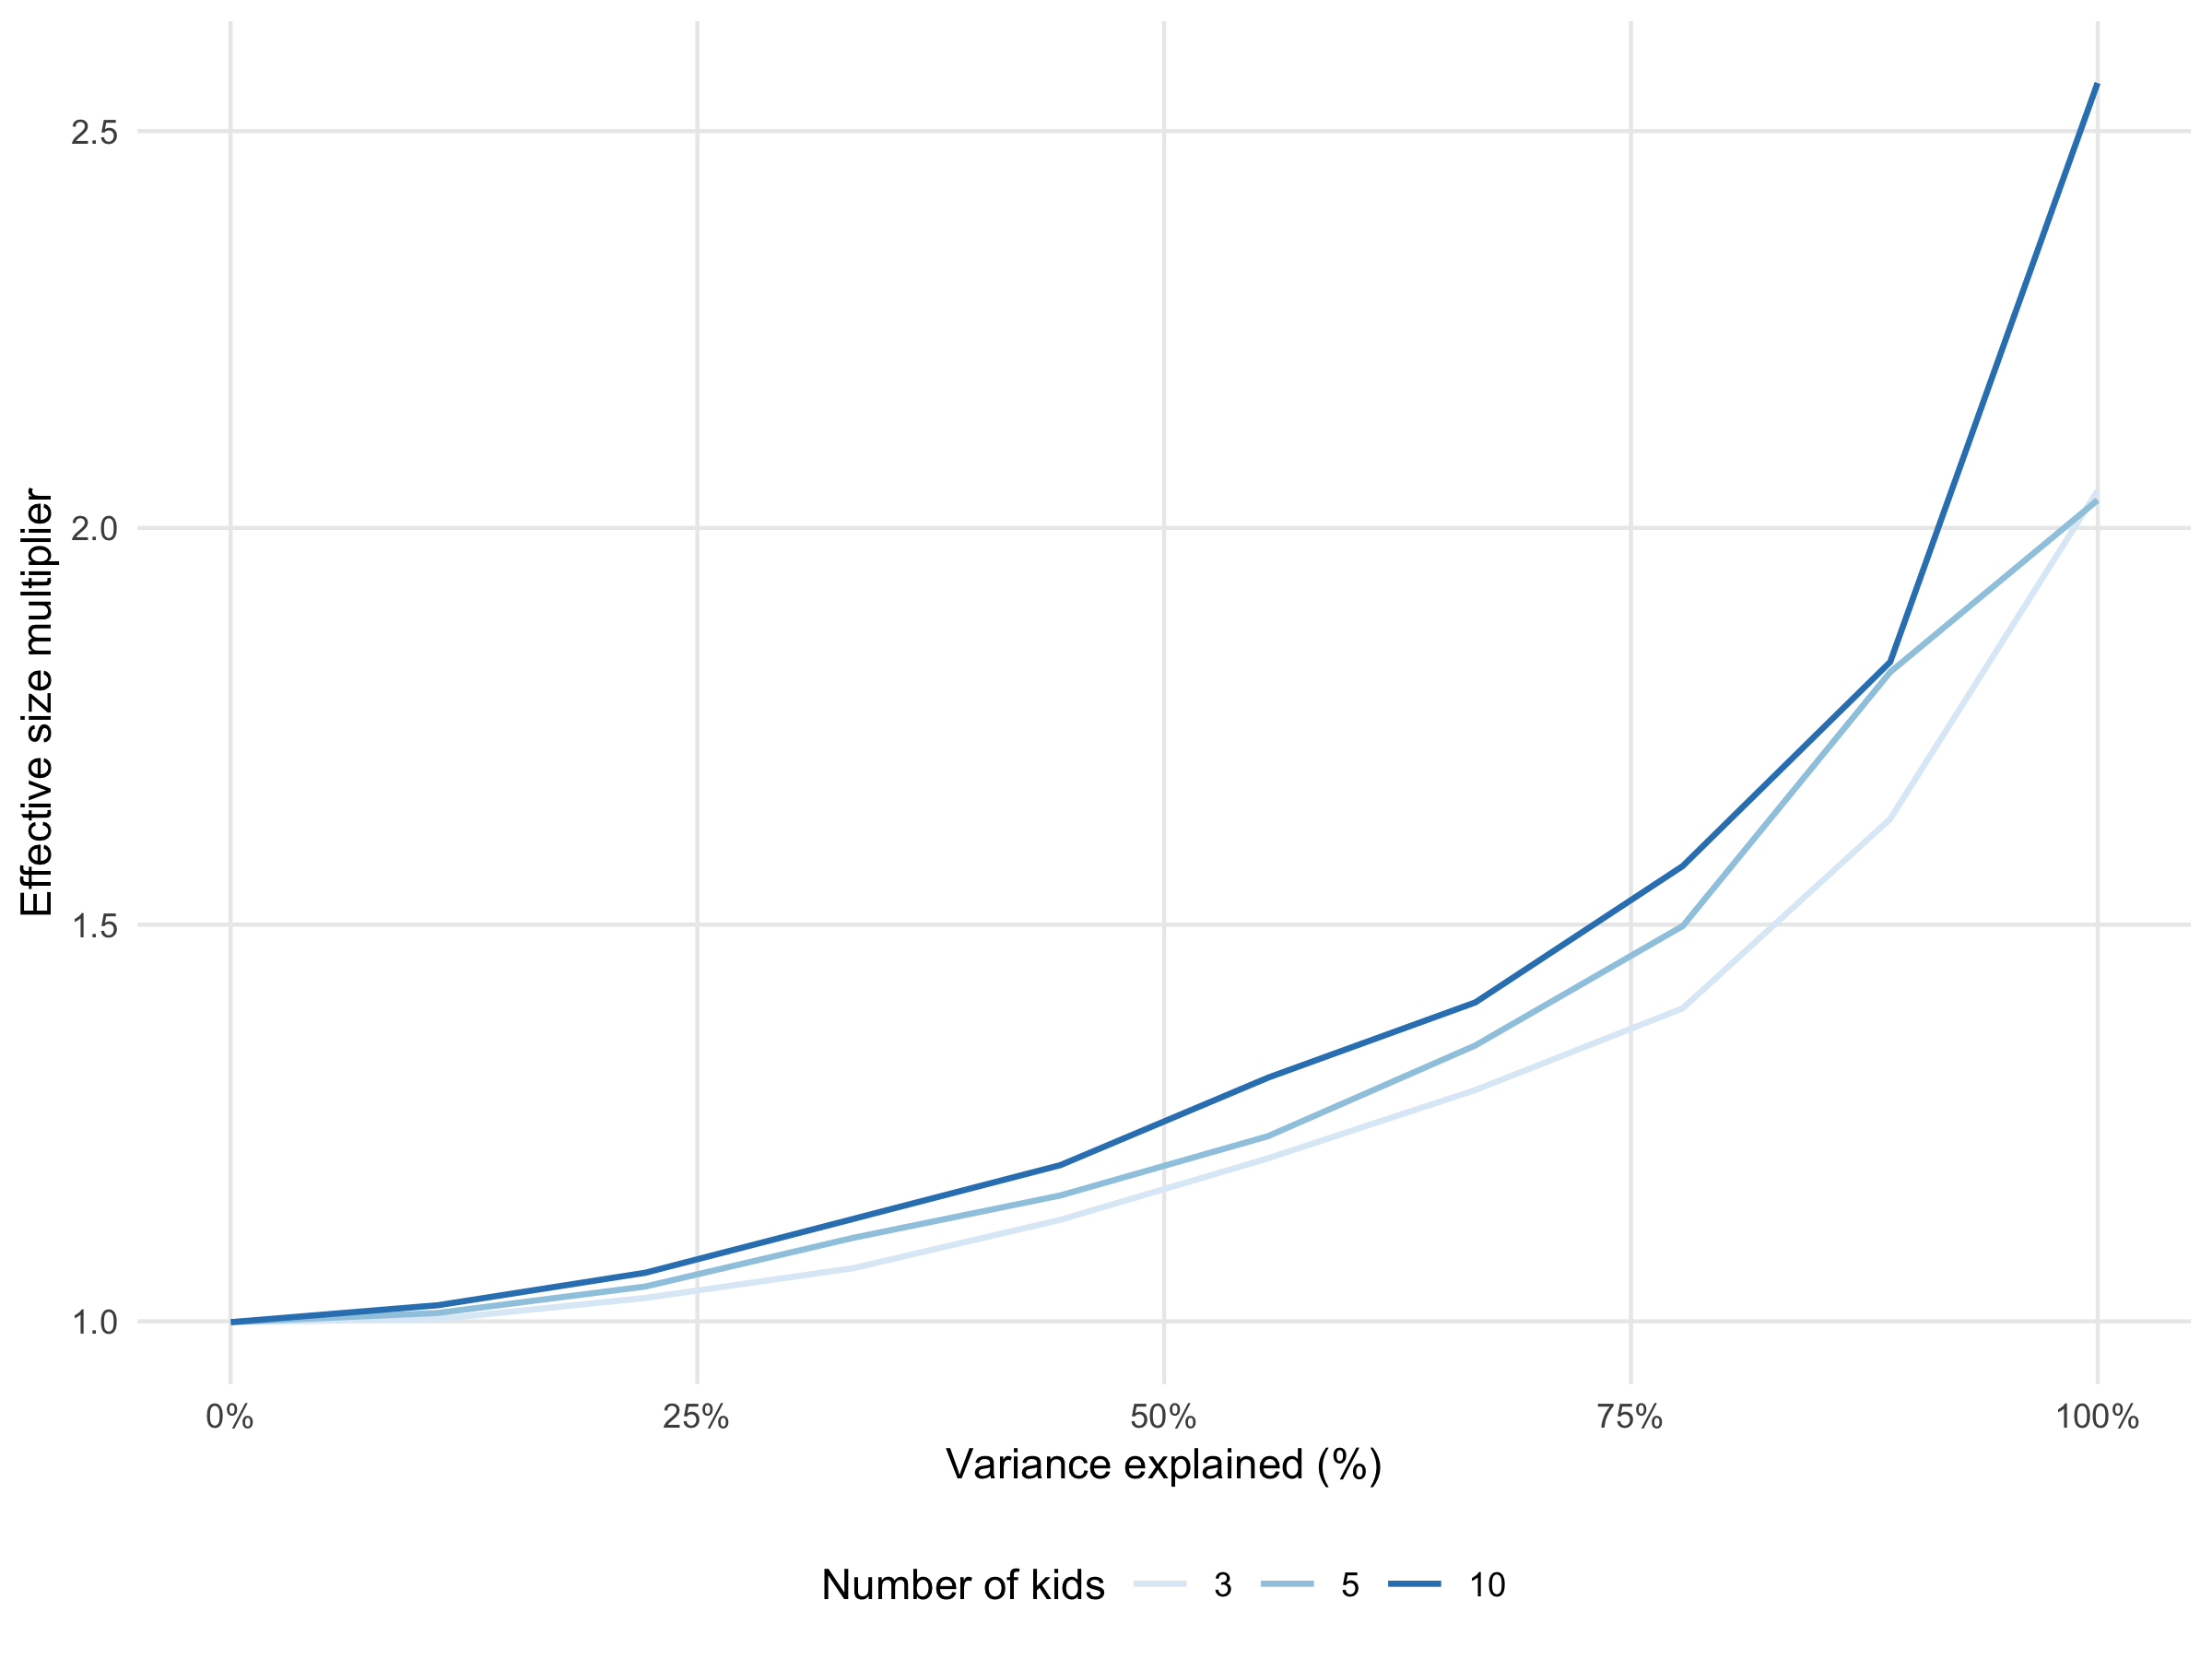
\includegraphics[width=1\linewidth]{figures/06-figure-sup-power-interaction-kids} 

}

\caption{Influence of family structure to detect
interaction genetic effect.}\label{fig:power-interaction-kids}
\end{figure}




\begin{figure}

{\centering 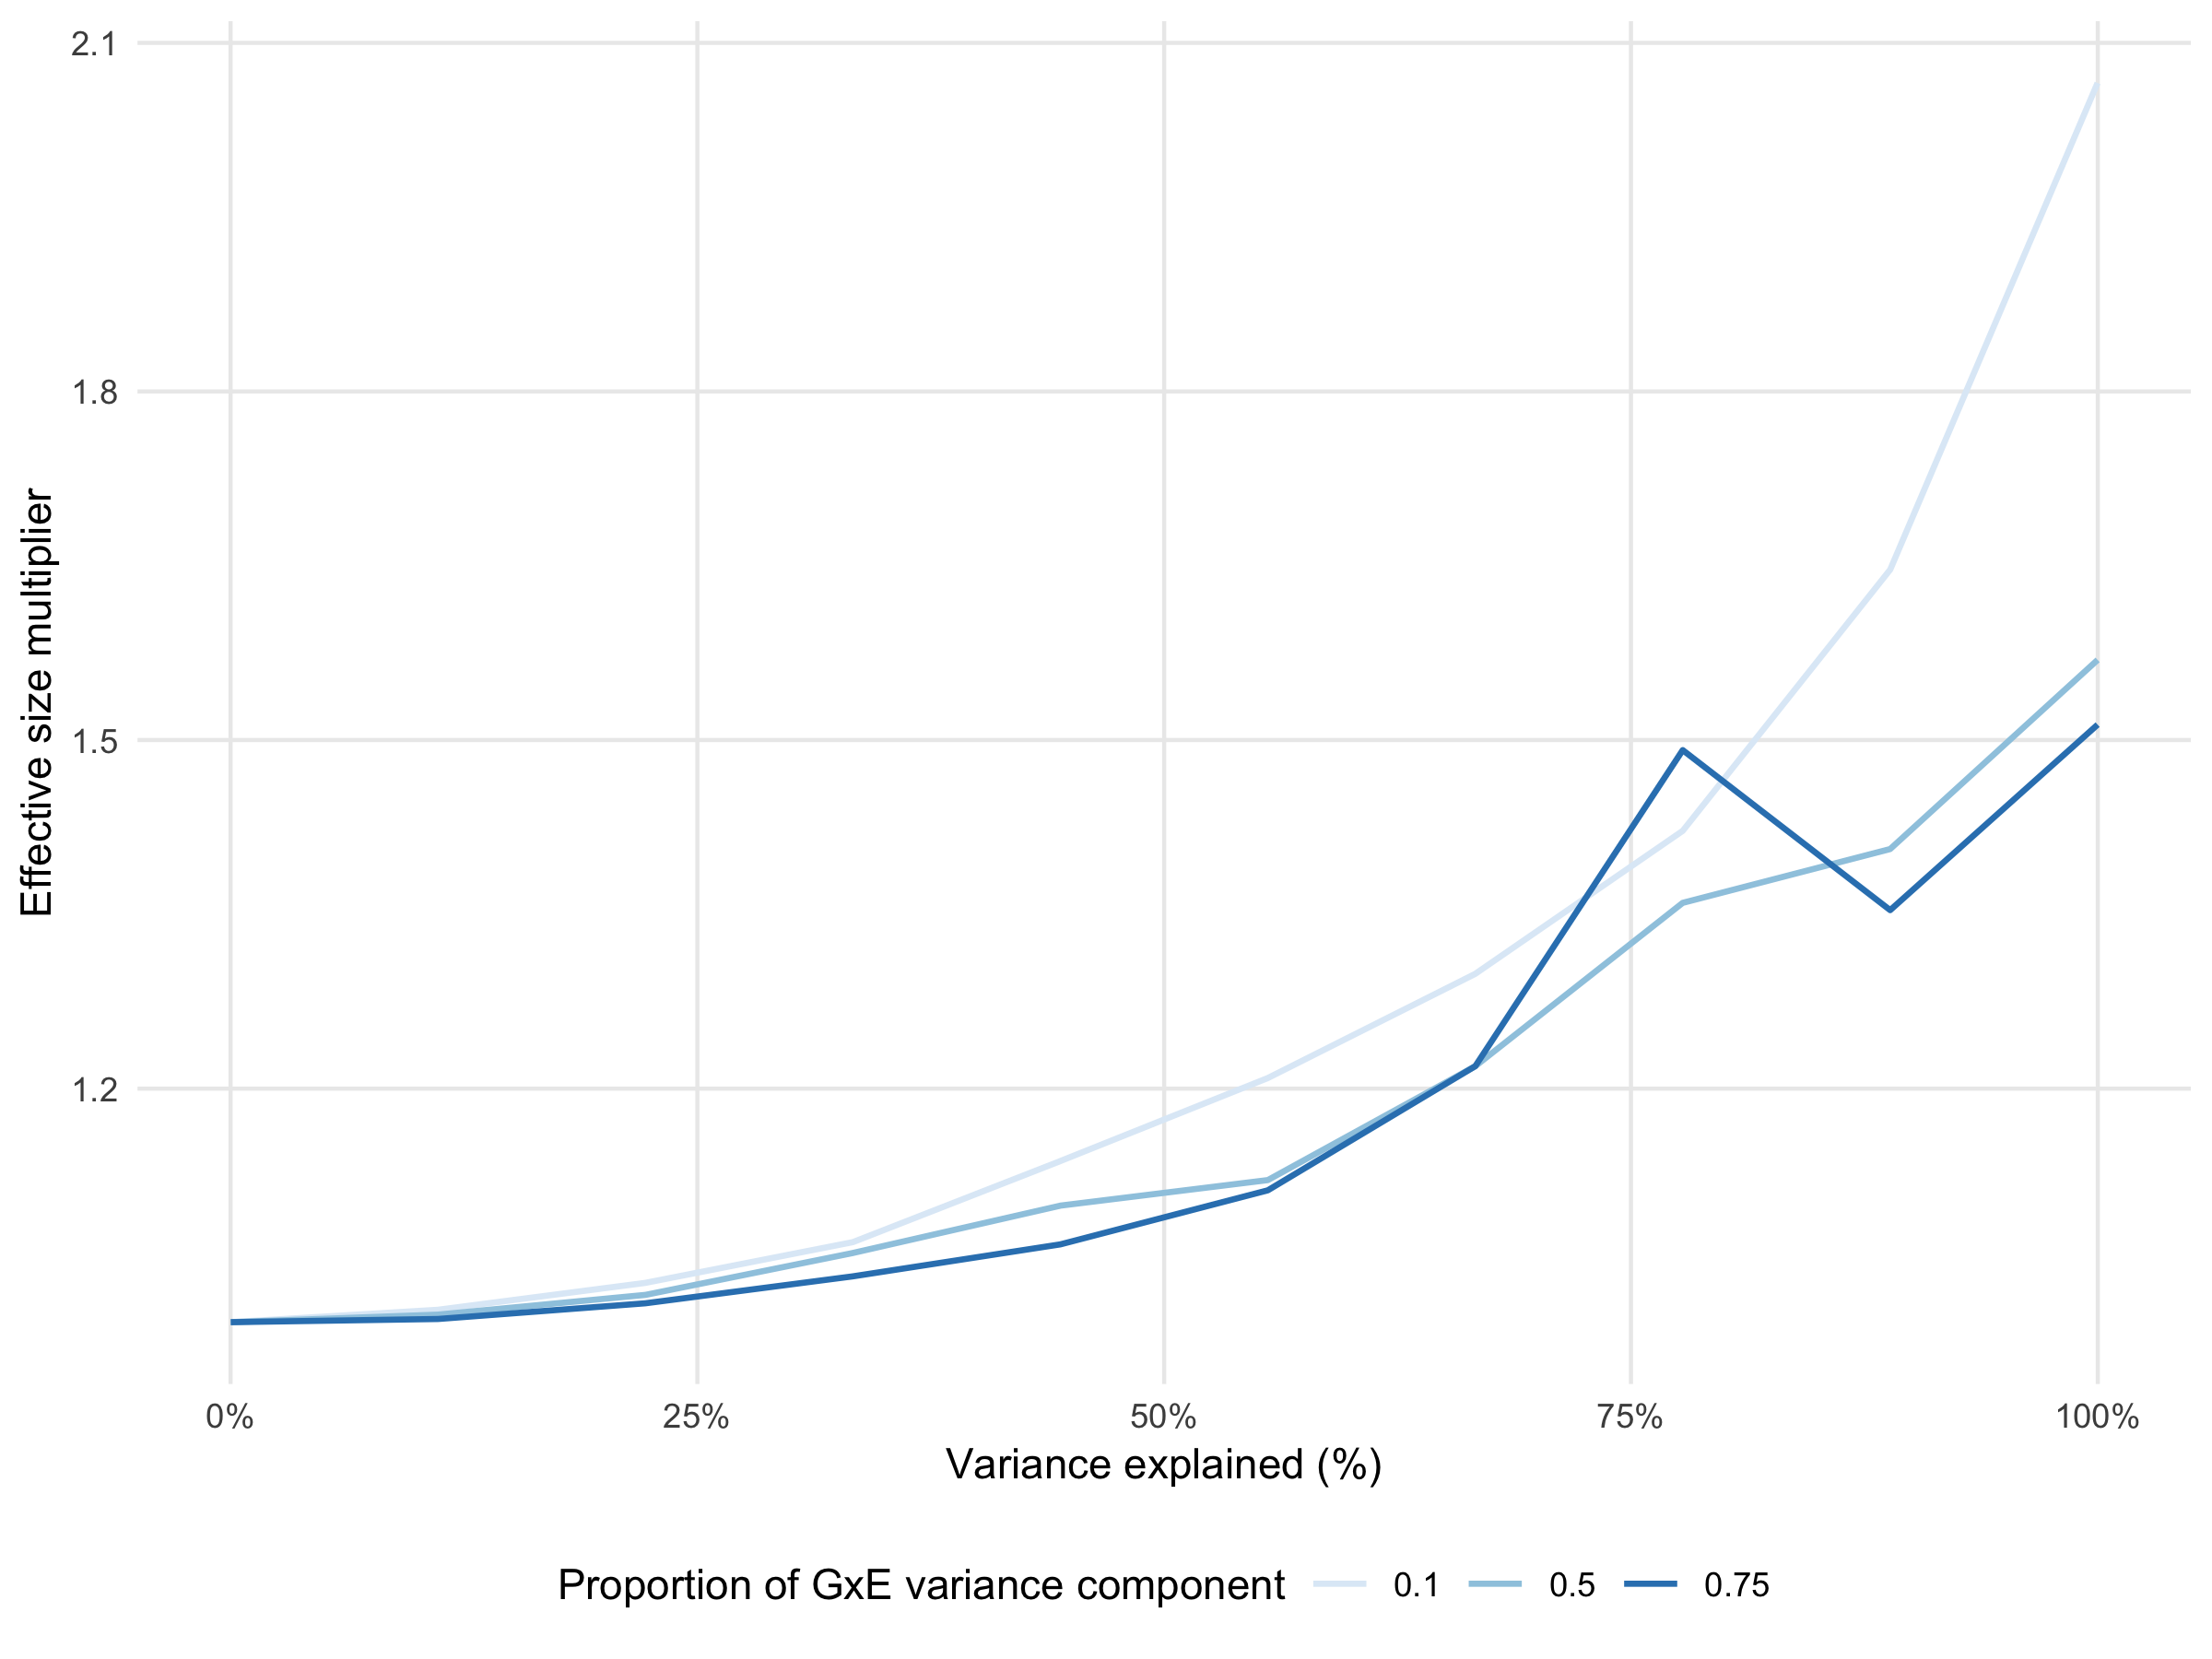
\includegraphics[width=1\linewidth]{figures/04-figure-sup-power-interaction-prop} 

}

\caption{Influence of GxE variance component to
detect interaction effect.}\label{fig:power-interaction-prop}
\end{figure}




\bibliography{gxefam.bib}

\backmatter
%\printindex

\end{document}
